% based on a template made by the university of cologne
% http://www.mi.uni-koeln.de/wp-MIEDV/wp-content/uploads/2016/07/LaTeX-Vorlage.zip - 2023-11-02
\documentclass[12pt,a4paper]{scrartcl}

\addtokomafont{sectioning}{\rmfamily}
\usepackage[ngerman]{babel}% deutsches Sprachpaket wird geladen
\usepackage[T1]{fontenc} % westeuropäische Codierung wird verlangt
\usepackage[utf8]{inputenc}% Umlaute werden erlaubt
\usepackage[usenames]{color} % Erlaubt die Benutzung der namen im Farbpaket und deren Änderung
\usepackage{amsmath} % Erweiterung für den Mathe-Satz
\usepackage{amssymb} % alle Zeichen aus msam und msmb werden dargestellt
\usepackage{graphicx} % Graphiken und Bilder können eingebunden werden
%\usepackage{multirow} % erlaubt in einer Spalte einer Tabelle die Felder in mehreren Zeilen zusammenzufassen
\usepackage{enumerate} % erlaubt Nummerierungen
\usepackage{xurl} % Dient zur Auszeichnung von URLs; setzt die Adresse in Schreibmaschinenschrift.
\usepackage[center]{caption}  % Bildunterschrift wird zentriert
%\usepackage{subfigure} % mehrere Bilder können in einer fugure-Umgebung verwendet werden
%\usepackage{longtable} % Diese Umgebung ist ähnlich definiert wie die tabular-Umgebung, erlaubt jedoch mehrseitige Tabellen.
%\usepackage{paralist} % Modifikation der bereits bestehenden Listenumgebungen
\usepackage{lmodern}% Für die Schrift
\usepackage[hidelinks]{hyperref} % Links und Verweise werden innerhalb von PDF Dokumenten erzeugt
%\usepackage{wrapfig} % Das Paket ermöglicht es von Schrift umflossene Bilder und Tabellen einzufügen.
\usepackage{latexsym} % LaTeX-Symbole werden geladen
\usepackage{tikz} % Erlaubt es mit tikz zu zeichnen
\usepackage{tabularx} % Erlaubt Tabellen
\usepackage{algorithm} % Erlaubt Pseudocode
\usepackage{color} % Farbpaket wird geladen
%\usepackage{stmaryrd} % St Mary Road Symbole werden geladen
\usepackage{physics}
\usepackage{mhchem} % Chemie: \ce & \pu

\numberwithin{equation}{section} % Nummerierungen der Gleichungen, die durch equation erstellt werden, sind gebunden an die section
\newcommand{\HRule}{\rule{\linewidth}{0.7mm}}
\newcommand{\pu}[1]{\ensuremath{\mathrm{#1}}}
\newcommand{\eqspaced}{\ensuremath{\;\;=\;\;}} % equal sign surrounded by spaces, used in align env to match eqnarray behaviour
\newcommand{\code}[1]{\textsf{#1}}

\hyphenation{An-samm-lung }
\hyphenation{auf-wen-dig}
\hyphenation{Brems-me-di-ums}
\hyphenation{be-schreibt}
\hyphenation{Cu-rie-Tem-pe-ra-tur}
\hyphenation{Dop-pel-ätz-me-tho-de}
\hyphenation{ei-ner-seits}
\hyphenation{ein-ge-stellt}
\hyphenation{e-lek-tro-mag-ne-tische}
\hyphenation{Ener-gie-stragg-ling}
\hyphenation{Ent-mag-neti-sier-ungs-fak-tor}
\hyphenation{Ent-mag-neti-sier-ungs-feld-stär-ke}
\hyphenation{Ent-mag-neti-sier-ungs-ver-hal-ten}
\hyphenation{Erd-be-schleu-ni-gung}
\hyphenation{Er-eig-nis-se}
\hyphenation{er-kenn-bar}
\hyphenation{er-rei-chen}
\hyphenation{ge-ra-der}
\hyphenation{Ge-schoss-e-ner-gi-en}
\hyphenation{Ge-schwin-dig-keit}
\hyphenation{Grenz-be-reich}
\hyphenation{Koh-len-stoff-ket-ten}
\hyphenation{Kom-mu-tie-rungs-kur-ve}
\hyphenation{konn-te}
\hyphenation{kor-ri-gier-te}
\hyphenation{Li-te-ra-tur-wer-te}
\hyphenation{Li-thi-um-fluo-rid-Kris-tal-len}
\hyphenation{Mag-ne-ti-sier-ungs-aus-rich-tung}
\hyphenation{nach-ge-wie-sen}
\hyphenation{nächs-ten}
\hyphenation{nä-he-rungs-wei-se}
\hyphenation{Nor-mal-ver-tei-lung}
\hyphenation{or-ga-ni-schen}
\hyphenation{Pri-mär-elek-tron}
\hyphenation{Scha-len-mo-dells}
\hyphenation{Schnitt-flä-che}
\hyphenation{Se-kun-där-elek-tron-en}
\hyphenation{Se-kun-där-elek-tron-en-ver-viel-fach-er}
\hyphenation{statt-fin-det}
\hyphenation{sys-te-ma-tisch-en}
\hyphenation{Ver-ar-mungs-zo-ne}
\hyphenation{vi-su-a-li-siert}
\hyphenation{Wie-der-ho-lung}
\hyphenation{zu-sätz-lich}


\hypersetup{
  pdftitle={B3.1},
  pdfcreator={LaTeX via pandoc}}

\setcounter{secnumdepth}{6}
\setcounter{tocdepth}{6}

\begin{document}
\begin{titlepage}
	\pagestyle{empty}

	\begin{center}

	\textsc{\LARGE Universität zu Köln }\\ [0.4cm]
	\textsc{Mathematisch-Naturwissenschaftliche Fakultät} \\[1.5cm]

	
\includegraphics[width=0.45\textwidth]{../media/uni.jpg}\\[1.5cm]  % Uni-Logo wird geladen

	\textsc{\Large Praktikum~B}\\[2mm]
	\textsc{}\\[10mm]
	\HRule \\[0.4cm]

		{	\Huge \bfseries B3.1}\\[0.4cm]
			{	\huge \bfseries Statistik der Kernzerfälle}\\[0.3cm]
	
	\HRule \\[3cm]

 	\begin{center}
		\textsc{\Large Catherine~Tran } \\[3pt]
		\textsc{\Large Carlo~Kleefisch } \\[3pt]
		\textsc{\Large Oliver~Filla } \\[3pt]
	\end{center}
	\end{center}
\end{titlepage}

\newpage
\tableofcontents
\newpage

\hypertarget{einleitung}{%
\section{Einleitung}\label{einleitung}}

In diesem Versuch wird die statistische Methode des $\chi^2$--Anpassungstests mithilfe von radioaktiver Strahlung untersucht. Dazu wird $\ce{^{137}Cs}$ verwendet, dessen Stahlung mit einem Geiger--Müller--Zählrohr detektiert wird.

Basierend auf den Messergebnissen werden drei Hypothesen über die Präperatsstärke bewertet. Zudem soll die Totzeit des Detektores milhilfe der Zwei--Präperate--Methode bestimmt werden.

\clearpage
\hypertarget{theoretische-grundlagen}{%
\section{Theoretische Grundlagen}\label{theoretische-grundlagen}}
\hypertarget{Radioaktiver Zerfall}{\subsection{Radioaktiver Zerfall}\label{Radioaktiver Zerfall}}
Bei radioaktivem Zerfall wandelt sich ein Atomkern in einen anderen Atomkern um, indem Teilchen ausgestoßen werden.

Es wird zwischen $(\alpha)$--, $\beta$--und $\gamma$--Zerfall unterschieden. Der Energiegewinn durch den Zerfall wird durch den $Q$--Wert beschrieben und kann durch die Weizsäcker Massenformel ermittelt werden.

\hypertarget{Halbwertszeit}{\subsubsection{Halbwertszeit}\label{Halbwertszeit}}
Die Halbwertszeit $T_{1/2}$ ist die Zeit, in der die Hälfte einer Anzahl von Kernen oder Elementarteilchen eines Stoffes zerfällt. Sie ist eine charakteristische Größe für radioaktive Zerfälle, die unabhängig von der aktuell vorhandenen Substanzmenge ist. \cite{Halbwertszeit}

\hypertarget{Zerfallswahrscheinlichkeit}{\subsubsection{Zerfallswahrscheinlichkeit}\label{Zerfallswahrscheinlichkeit}}
Die \emph{Zerfallswahrscheinlichkeit} $\alpha$ ist eine isotopspezifische Konstante, die angibt wie schnell ein Kern des entsprechenden Isotops zerfällt. Sie steht in Relation mit der Halbwertszeit $T_{1/2}$. Dies wird im folgenden Abschnitt hergeleitet.

\begin{eqnarray}
	\alpha &=& \frac{\ln{(2)}}{T_{1/2}} \label{eq:Zerfallswahrscheinlichkeit}
\end{eqnarray}

\noindent
Das in diesem Versuch verwendete $\ce{^{137}Cs}$ hat eine Halbwertszeit von $T_{1/2}\approx30.08\mathrm{\,a}$ \cite{Chart of Nuclides}, was etwa $9.49 \cdot 10^8 \mathrm{\,s}$ entspricht. Daraus kann die Zerfallswahrscheinlichkeit $\alpha$ nach \eqref{eq:Zerfallswahrscheinlichkeit} bestimmt werden.

\begin{eqnarray}
	\alpha_\mathrm{Cs} &\approx& 7.3 \cdot 10^{-10} \mathrm{\,s^{-1}}
\end{eqnarray}

\hypertarget{Herleitung Zerfallswahrscheinlichkeit}{\subsubsection{Herleitung der Zerfallswahrscheinlichkeit}\label{Herleitung Zerfallswahrscheinlichkeit}}
Ein instabiler Kern mit einer Halbwertszeit $T_{1/2}$ zerfällt mit einer Wahrscheinlichkeit $\omega$ innerhalb einer Zeitspanne $\Delta t$. Falls diese Zeitspanne $\Delta t$ klein gegen $T_{1/2}$ ist, lässt $\omega$ linear annähern. Die Gegenwahrscheinlichkeit $(1-\omega)$ beschreibt demnach den Fall, dass der Kern nicht zerfällt.

\begin{eqnarray}
	\omega &=& \alpha \Delta t \label{eq:Zerfallswkt linear} \\
	1 - \omega &=& 1 - \alpha \Delta t
\end{eqnarray}

\noindent
Nun sollen größere Zeitspannen $t$ betrachtet werden. Dazu wird $t$ so in $k$ gleich große Teilzeitspannen unterteilt, dass jede Teilzeitspanne $t_i$ klein genug ist, um linear angenähert zu werden. Dann kann die Wahrscheinlichkeit $(1 - \omega_i)$ dafür ermittelt werden, dass in der Teilzeitspanne $t_i$ kein Zerfall stattfindet \eqref{eq:t_i kein zerfall}.

Daraus kann die Wahrscheinlichkeit $(1 - \omega)$ für den Erhalt des Kerns nach der Zeit $t$ ermittelt werden \eqref{eq:t kein zerfall}.

\begin{eqnarray}
	1 - \omega_i &=& \left(1 - \alpha \frac{t}{k}\right) \label{eq:t_i kein zerfall} \\
	1 - \omega &=& \left(1 - \alpha \frac{t}{k} \right)^k \label{eq:t kein zerfall}
\end{eqnarray}

\noindent
Um ein exaktes Ergebnis zu erzielen, müssen die Teilzeitabschnitte infinitesimal klein sein. Damit wird $k$ unendlich groß. Dadurch kann die Wahrscheinlichkeit $(1-\omega)$ für den Erhalt des Kerns durch eine Exponentialfunktion beschrieben werden.

Ensprechend kann die Wahrscheinlichkeit $\omega$ für einen Zerfall innerhalb der Zeitspanne $t$ beschrieben werden.

\begin{eqnarray}
	1 - \omega &=& \lim_{k \rightarrow \infty} \left(1 - \alpha \frac{t}{k} \right)^k \\
		&=& e^{- \alpha t} \\
	\omega &=& 1 - e^{-\alpha t}
\end{eqnarray}

\noindent
Die Zerfallswahrscheinlichkeit $\alpha$ lässt sich nun aus der Halbwertszeit ermitteln.

\begin{eqnarray}
	\omega(T_{1/2}) &=& \frac{1}{2} \\
	\Rightarrow\alpha &=& \frac{\ln{(2)}}{T_{1/2}}
\end{eqnarray}

\hypertarget{statistik}{\subsection{Statistik}\label{statistik}}

\subsubsection{Zufallsvariablen}
\label{Zufallsvariablen}
Eine \emph{Zufallsvariable} ist eine Funktion $X$, die jedem Ereignis $\omega$ eines Zufallsexperiments eindeutig eine reelle Zahl zuordnet. Sie kann sowohl diskret als auch kontinuierlich sein.

\begin{eqnarray}
	X : \omega \rightarrow x(\omega) \in \mathbb{R}
\end{eqnarray}

\noindent
Das Ereignis $\omega$ des Zufallsexperiments kann direkt eine Zahl sein, wie beispielsweise die Augenzahl eines Würfelswurfs. Alternativ kann Jedem Ereignis des Zufallsexperiments wird eine Zahl zugeordnet werden, beispielsweise können bei einem Münzwurf dem Ereignis $\mathrm{Kopf}$ der Wert $0$ und dem Ereignis $\mathrm{Zahl}$ eine $1$ zugeordnet werden.

\subsubsection{Wahrscheinlichkeitsdichte}
\label{Wahrscheinlichkeitsdichte}
Eine \textit{Wahrscheinlichkeitsdichte} (PDF\footnote{\emph{Probability Density Function}}) ist eine Funktion $f(y)$, welche die Wahrscheinlichkeit $\mathbb P$ angibt, dass eine Zufallsvariable $X$ einen Wert innerhalb eines Intervalls $[a,b]$ annimmt.

\begin{eqnarray}
	\int_{a}^{b} f(y) dy &=& \mathbb P(X(\omega) \in [a,b])
	\label{eq:wahrscheinlichkeitsdichte}
\end{eqnarray}

\noindent
Die Wahrscheinlichkeitsdichte kann auch Werte über $1$ annehmen. Beispielsweise kann der Ort eines Punktteilchens durch eine $\delta$-Funktion beschrieben werden. Im Fall von diskreten Zufallsvariablen kann auch die Wahrscheinlichkeitsdichte diskret sein.

\subsubsection{Wahrscheinlichkeitsverteilung}
\label{Wahrscheinlichkeitsverteilung}
Eine \emph{Wahrscheinlichkeitsverteilungsfunktion} (CDF\footnote{\emph{Cumulative Distribution Function}, kumulative Verteilungsfunktion}) einer Zufallsvariable $X$ ist dagegen eine Funktion $F(y)$, die angibt mit welcher Wahrscheinlichkeit $\mathbb P$ die Zufallsvariable $X$ einen Wert kleiner gleich $y$ annimmt. Sie ist die integrierte Wahrscheinlichkeitsdichte $f(\omega)$.

\begin{eqnarray}
	F(y) &=& \mathbb P(X(\omega) \leq y) \\
	F(y) &=& \int_{- \infty}^{y} f(\tilde{y}) d\tilde{y}
\end{eqnarray}

\subsection{Wahrscheinlichkeitsverteilungen}
\label{Wahrscheinlichkeitsverteilungen}

\subsubsection{Binomialverteilung}
\label{Binomialverteilung}
Die \emph{Binomialverteilung} ist eine wichtige diskrete Wahrscheinlichkeitsverteilung. Sie beschreibt ein Zufallsexperiment, das genau zwei sich gegenseitig ausschließende Ereignisse $A$ und $B$ haben kann. Die entsprechenden Wahrscheinlichkeiten $\mathbb P$ können wie folgt definiert werden.

\begin{eqnarray}
	\mathbb P(A) &=& p \\
	\mathbb P(B) &=& 1 - p
\end{eqnarray}

\noindent
Dieses Experiment wird $N$-mal durchgeführt, wobei die einzelnen Ergebnisse jeder Wiederholung unabhängig von den Ergebnissen der vorherigen Wiederholungen sind. Die Zufallsvariable $X$ gibt dann die Anzahl $n$ an eingetretenen Ereignissen $A$ an. Dabei spielt die Reihenfolge, in der die Ereignisse $A$ eintreten, keine Rolle.

Die entsprechende  Wahrscheinlichkeit $P(N,n,p)$ gibt demnach die Wahrscheinlichkeit an, dass das Ereignis $A$ genau $n$-mal eintritt. Weiterhin können der Erwartungswert $\mu$ und die Varianz $\sigma^2$ bestimmt werden.

\begin{eqnarray}
	P(N,n,p) &=& \binom{N}{n} p^n (1-p)^{N-n} \\
	m_B &=& Np \\
	\sigma^2_B &=& N p (1-p)
\end{eqnarray}

\noindent
Der Binomialkoeffizient $\binom{N}{n}$ dient dabei dazu, alle möglichen Reihenfolgen zu berücksichtigen, in der das Ereignis $A$ eintreten kann, wobei der restliche Term die Wahrscheinlichkeit angibt, dass das Ereignis $A$ in einer bestimmten Reihenfolge $n$-mal eintritt.

\subsubsection{Poissonverteilung}
\label{Poissonverteilung}
Die \emph{Poissonverteilung} beschreibt Reihen von Zufallsvariablen, die unabhängig voneinander eintreten. Sie ist eine weitere diskrete Verteilung mit der Wahrscheinlichkeitsdichte $P(n,\lambda)$, Erwartungswert $m$ und Varianz $\sigma^2$.

\begin{eqnarray}
	P_\lambda(n) &=& \frac{\lambda^n}{n!} e^{-\lambda}
	\label{eq:poisson} \\
	m &=& \lambda\\
	\sigma^2 &=& \lambda \\
	\Rightarrow\quad \frac{\sigma}{m} &=&\frac{1}{\sqrt{m}} \label{eq:Poisson STD/EW}
\end{eqnarray}

\noindent
Die Poissonverteilung $P_\lambda(n)$ folgt als Grenzfall aus der Binomialverteilung $P(N, n, p)$ mit infinitesimal kleinen Schrittgrößen $(p\rightarrow 0)$ und unendlich vielen Schritten $(N\rightarrow 0)$. Dabei bildet $\lambda\equiv Np$ eine Konstante. Die Poissonverteilung ist als Näherung für die Binomialverteilung zu verwenden, falls folgende Bedingung erfüllt ist.

\begin{eqnarray}
	P(n, \lambda)  &=& \lim_{N \rightarrow \infty \atop p\rightarrow 0} P(N, n, p) \\
	m_B &\leq& 10
\end{eqnarray}

\subsubsection{Gaußverteilung}
\label{Gaußverteilung}
Die \emph{Gaußverteilung} ist eine kontinuierliche Verteilung. Ihre Wahrscheinlichkeitsdichte $P(x,\mu,\sigma)$ wird folgendermaßen mithilfe des Erwartungswerts $\mu$ und der Varianz $\sigma^2$ beschrieben. Die \emph{Normalverteilung}  ist eine Gaußverteilung mit $\mu=\sigma^2=1$.

\begin{eqnarray}
	P(x,\mu,\sigma) &=& \frac{1}{\sqrt{2 \pi\sigma^2}} \exp\left[- \frac{1}{2} \left(\frac{x - \mu}{\sigma}\right)^2\right]
\end{eqnarray}

\noindent
Der Grenzwert der Poissonverteilung für $\lambda \rightarrow \infty$ liefert die Gaußverteilung.

\begin{eqnarray}
	\lim_{\lambda \rightarrow \infty} \frac{\lambda^n e^{-\lambda}}{n!} = \frac{1}{\sqrt{2 \pi \lambda}} e^{- \frac{(x-\lambda)^2}{2\lambda}}
\end{eqnarray}

\noindent
Weiterhin konvergiert die Binomialverteilung nach dem \emph{Satz von Moivre--Laplace} für $N \rightarrow \infty$ mit der Bedingung $0 < p < 1$ gegen die Normalverteilung. Eine Faustregel besagt, dass die Normalverteilung schon eine gute Näherung für die Binomialverteilung liefert, sobald ihre Varianz $\sigma^2_B$ mindestens $9$ beträgt.

\begin{eqnarray}
	\lim_{N \rightarrow \infty} \binom{N}{n} p^n (1-p)^{N-n}
		&=& \frac{1}{\sqrt{2 \pi N p (1-p)}} e^{- \frac{(x - Np)^2}{2 N p (1-p)}} \\
	\sigma^2_B &\geq& 9
\end{eqnarray}

\hypertarget{Intervallverteilung}{\subsection{Intervallverteilung}\label{Intervallverteilung}}
Die \emph{Intervallverteilung} ist dann gefragt, wenn nicht die Anzahl an eingetroffenen Ereignissen $A$, sondern stattdessen die Zeit zwischen zwei oder mehr Ereignissen $A$ interessant ist.

Für Kernzerfälle ist ihre Wahrscheinlichkeitsdichte $P_n$ wie folgt gegeben. Sie ähnelt der Poissonverteilung, hat aber einen zusätzlichen Faktor $a$.

\begin{eqnarray}
	P_n &=& a \frac{(at)^n}{n!} e^{-at} \label{eq:Intervallverteilung}
\end{eqnarray}

\noindent
Damit gibt die kumulative Verteilungsfunktion $\int_{t_0}^{t_1} P_n \,\mathrm dt \label{eq:P_n_int}$ die Wahrscheinlichkeit an, dass in dem Zeitintervall $[t_0,t_1]$ zwei Ereignisse im Abstand $t$ stattgefunden haben, sowie $n$ weitere Ereignisse zwischen diesen beiden. Somit haben in der Zeit $t$ exakt $n+2$ Ereignisse stattgefunden.

Somit gibt die Verteilungsfunktion für $n=0$ die Wahrscheinlichkeit an, dass die Zeit $t$ zwischen zwei aufeinanderfolgenden Zerfällen innerhalb des Intervalls $[t_0, t_1]$ liegt.

\hypertarget{Herleitung Intervallverteilung}{\subsection{Herleitung}\label{Herleitung Intervallverteilung}}
Nun soll die Wahrscheinlichkeitsdichte $P_n$ der Intervallverteilung hergeleitet werden.

Hierzu wird die Wahrscheinlichkeit $W$ bestimmt, dass die Zeit zwischen zwei Zerfällen, zwischen denen genau $n$ andere Zerfälle stattfinden, den Wert $\Delta t$ annimmt. $W$ setzt sich aus dem Produkt zweier Einzelwahrscheinlichkeiten $W_1$ und $W_2$ zusammen.

$W_1$ gibt die Wahrscheinlichkeit an, dass im Zeitintervall $\Delta t$ genau $n$ weitere Zerfälle stattfinden. Dies wird durch eine Poissonverteilung \eqref{eq:poisson} beschrieben, deren Erwartungswert $\lambda = a\Delta t$ beträgt und durch die Zerfallswahrscheinlichkeit $a$ beschrieben wird.

$W_2$ hingegen gibt die Wahrscheinlichkeit an, dass nach der Zeit $\Delta t$ in einer sehr kurzen Zeit $\mathrm dt$ ein Zerfall stattfindet. Aufgrund der kurzen Zeitspanne kann dies linear genähert werden, wie es bei der Herleitung der Zerfallswahrscheinlichkeit in Abschnitt \ref{Herleitung Zerfallswahrscheinlichkeit}  in Gleichung \eqref{eq:Zerfallswkt linear} gemacht wurde.

\begin{eqnarray}
	W_1 &=& \frac{(a\Delta t)^n}{n!} \mathrm{e}^{-a\Delta t} \\
	W_2 &=& a \,\mathrm dt \\
	W &=& W_1 \cdot W_2 \\
		&=& \frac{\left(a\Delta t\right)^n}{n!}  \mathrm{e}^{-a\Delta t} \cdot a \,\mathrm dt
\end{eqnarray}

\noindent
Da die Wahrscheinlichkeit $W$ das Integral der Wahrscheinlichkeitsdichte $P_n$ darstellt, wird $P_n$ durch differenzieren ermittelt.

\begin{eqnarray}
	P_n &=& \frac{\mathrm dW}{\mathrm dt} \\
		&=& a \frac{\left(at\right)^n}{n!} e^{-at}
\end{eqnarray}

\hypertarget{statistische-tests}{%
\subsection{Statistische Tests}\label{statistische-tests}}

\hypertarget{hypothesentest}{%
\subsubsection{Hypothesentest}\label{hypothesentest}}

Ein Hypothesentest oder Statistischer Test dient dazu, durch eine Hypothese mittels statistischer Messungen zu bewerten.

Dazu verwendet man eine \emph{Nullhypothese}\footnote{\emph{Hypothesis  to be nullified} \cite{Gigerenzer}} $H_0$ und eine \emph{Gegenhypothese} oder \emph{Alternativhypothese} $H_1$, die sich unterscheiden. Ziel des Tests ist es, die Alternativhypothese $H_1$ zu belegen. Falls dies nicht gelingt, muss man die Nullhypothese $H_0$ als wahr annehmen. Diese wird nicht überprüft. \cite{Statistical Inference}

Aufgrund der Zufälligkeit der Ereignisse kann es dabei zwei Arten von Fehlern geben. Ein $\alpha$--Fehler beschreibt das irrtümliche Ablehnen von $H_0$, während ein $\beta$--Fehler das fälschliche Annehmen von $H_0$ bezeichnet.

\hypertarget{fehlerarten}{%
\subsubsection{Fehlerarten}\label{fehlerarten}}
Ein \emph{Fehler erster Art} oder $\alpha$--Fehler beschreibt die fälschliche Ablehnung der Nullhypothese $H_0$ in einem Statistischen Test. Man nimmt z.B. an, dass ein Würfel gezinkt ist $(H_1)$, obwohl er in Wahrheit fair ist $(H_0)$. Hierbei ist die $H_0$ die Annahme eines fairen Würfels. Man spricht hier auch von einem \emph{falsch--positiven} Ergebnis. \cite{Statistical Inference}

Ein \emph{Fehler zweiter Art} oder \emph{$\beta$--Fehler} beschreibt umgekehrt die fälschliche Akzeptanz der Nullhypothese $H_0$. Beispielsweise geht man davon aus, dass ein Würfel fair ist $(H_0)$, obwohl er tatsächlich unfair ist $(H_1)$. Man spricht hier auch von einem \emph{falsch--negativen} Ergebnis. \cite{Statistical Inference}

Die statistische Signifikanz beschreibt die erlaubte Wahrscheinlichkeit, einen $\alpha$--Fehler zu begehen. \cite{Statistical Inference} In einem \emph{Alternativtest} dagegen beschreibt die Signifikanz die Wahrscheinlichkeit, einen $\alpha$- oder einen $\beta$--Fehler zu machen. Bei einer Signifikanz $Y$ sind $\alpha$-- und $\beta$--Fehler mit einer Wahrscheinlichkeit von je $\frac{Y}{2}$ erlaubt.

\hypertarget{der-chi2anpassungstest}{%
\subsubsection{\texorpdfstring{Der
$\chi^2$--Anpassungstest}{Der \textbackslash chi\^{}2--Anpassungstest}}\label{der-chi2anpassungstest}}

Der $\chi^2$--Anpassungstest dient dazu, eine Verteilung von Zufallsvariablen $A$ mit einer theoretischen Verteilung zu vergleichen. Man kann mithilfe des Tests bewerten, ob die Zufallsvariablen der Verteilung entsprechen können. Hierbei werden sowohl Fehler 1. Art als auch Fehler 2. Art berücksichtigt.

Die Grundidee dahinter ist, einen Erwartungswert $\expval{A}$ und seine Varianz $\sigma_A^2$ bewerten zu können. Das Maß für die Abweichung von der Hypothese wird für einen Freiheitsgrad durch $\chi^2$ beschrieben,\footnote{Man könnte auch den Betrag $|x_i|$   anstatt des Quadrates $x_i^2$ wählen. Dies wird nicht gemacht, weil   damit schwieriger zu rechnen ist.} was durch die $\chi^2$--Verteilung beschrieben wird.

\begin{eqnarray}
    \chi^2 &=& \sum_i x_i^2
\end{eqnarray}

Mithilfe der $\chi^2$--Verteilung kann eine Signifikanz $Y$ festgelegt werden. Damit kann ein Intervall $[\chi^2_\mathrm{min}, \chi^2_\mathrm{max}]$ durch die Verteilungsfunktion $F(x, f)$ ermittelt werden. Liegt das ermittelte $\chi^2$ in diesem Interval, so kann $H_1$ als signifikant gültig angenommen werden.

\begin{eqnarray}
    F(\chi^2_\mathrm{min}, f) &=& 1 - \frac{Y}{2} \\
    F(\chi^2_\mathrm{max}, f) &=& \frac{Y}{2}
\end{eqnarray}

Oft wird die Signifikanz von $Y=5\,\%$ gefordert, wodurch das Gültigkeitsintervall durch folgende Gleichungen bestimmt wird.

\begin{eqnarray}
    F(\chi^2_\mathrm{min}, f) &=& 0.975 \label{eq:ChiMinFormula} \\
    F(\chi^2_\mathrm{max}, f) &=& 0.025 \label{eq:ChiMaxFormula}
\end{eqnarray}

Falls $\chi^2<\chi^2_\mathrm{min}$ das Ergebnis des Tests ist, sind die Daten zu gut an die These angepasst. Dies kann beispielsweise durch Overfitting entstehen.

\hypertarget{pearsons-chi2test}{%
\paragraph{\texorpdfstring{Pearsons
$\chi^2$--Test}{Pearsons \textbackslash chi\^{}2--Test}}\label{pearsons-chi2test}}

Eine Variante des $\chi^2$--Tests betrachtet nur ein Ende der Gauß--Verteilung. Hierbei wird die Signifikanz $Y$ verwendet, um ein maximal gültiges $\chi_\mathrm{max}^2$ zu bestimmen, dabei wird auf einen minimalen Wert verzichtet. \cite{McHugh} Damit kann eine Hypothese nur dann abgelehnt werden, wenn $\chi^2$ zu groß ist, ein zu kleines $\chi^2$ ist dabei nicht betrachtet. Auch hier wird oft eine Signifikanz von $5\,\%$ verwendet.

\begin{eqnarray}
    F(\chi^2_\mathrm{max}, f) &=& Y \\
    F(\chi^2_\mathrm{max}, f) &=& 0.05 \label{eq:ChiMaxPearson} \\
\end{eqnarray}

\hypertarget{die-chi2verteilung}{%
\subsubsection{Die $\chi^2$--Verteilung}\label{die-chi2verteilung}}

Sei $A$ standardnormalverteilt\footnote{Diese Annahme ist bei ausreichend vielen Messung durch das Gesetz der großen Zahl gerechtfertigt.}, dann ist die $\chi_1^2$--Verteilung eine quadrierte Normalverteilung mit einem Freiheitsgrad. Daher ist der Erwartungswert $\expval{\chi_1^2}=1$. Gibt es mehrere Freiheitsgrade $f$, so müssen $f$ Erwartungswerte $\expval{\chi_i^2}$ addiert werden, um den gesamten Erwartungswert zu ermitteln. Dies wird durch die Wahrscheinlichkeitsdichte (PDF\footnote{\emph{probability density function}}) $f(x, f)$ beschrieben,\footnote{Achtung: Hier wird zur besseren Lesbarkeit $f(x, 2f)$ angegeben, die Zahl der Freiheitsgrade wird in der Funktion halbiert.} wobei die Gammafunktion $\Gamma(x)$ benötigt wird.

\begin{eqnarray}
    f(x, 2f) &=&
        \begin{cases}
                \frac{x^{f-1}}{2^f}
                    \frac{\exp[-\frac{x}{2}]}{\Gamma(f)}
                    & : x\ge 0 \\
                0 & : x < 0
        \end{cases} \\
    \Gamma(x) &=& \int_0^\infty t^{x-1}\cdot \mathrm e^t \,\mathrm dt
\end{eqnarray}

Die Verteilungsfunktion (CDF\footnote{\emph{cumulative distribution function}}) $F(x, f)$ ist dabei komplex und hat den Erwartungswert $\expval{\chi_f^2}=f$ und die Varianz $\sigma_{\chi^2}=2f$.

\begin{align}
    F(x, 2f) &=
        \int_0^x
            \frac{y^{f-1}}{2^f}
                \frac{\exp[-\frac{y}{2}]}{\Gamma(f)}
            \,\mathrm dy \\
    \expval{\chi_f^2} &=
        \int_0^\infty x\cdot f(x, f)
            \,\mathrm dx
        &&= f \\
    \sigma_{\chi^2} &=
        \int_0^\infty \left(x - \expval{\chi_f^2}\right)^2 \cdot f(x, f)
            \,\mathrm dx
         &&=2f
\end{align}

\hypertarget{versuchsidee}{%
\subsection{Versuchsidee}\label{versuchsidee}}

In diesem Versuch wird $\ce{^{137}Cs}$ als radioaktive Probe verwendet, das eine Halbwertszeit $t_\frac{1}{2}\approx 30\,\mathrm a$ hat.

Damit soll die folgende Hypothese getestet, die Präparatstärke sei konstant und habe den Wert $\bar n$. Hierbei ist $\bar n$ der Mittelwert von vielen Einzelmessungen $n_i$ über eine kurze Zeit von $\Delta t=20\,\mathrm s$, der durch Gleichung $\eqref{mittlereRate}$ bestimmt wird. All diese $N$ Messungen werden in einem Zeitraum von wenigen Stunden absolviert.

Da der Zeitraum der Messungen sehr kurz gegen die Halbwertszeit ist, kann man annehmen, dass die Stärke der Probe sich im Rahmen der Messungenauigkeit nicht verändert.

Damit können die Differenzen zum Mittelwert $(n_i-\bar n)$ ermittelt werden. Nach dem zentralen Grenzwertsatz sind die relativen Differenzen standardnormalverteilt. Dadurch kann die Abweichung $\chi^2$ wie folgt ermittelt werden.

\begin{eqnarray}
    \bar n &=& \sum_{i=1}^N \frac{n_i}{N} \label{mittlereRate} \\
    \chi^2 &=& \sum_{i=1}^N \frac{(n_i-\bar n)^2}{\bar n} \label{ChiSquared}
\end{eqnarray}

\subsubsection{Das Geiger--Müller--Zählrohr}
\label{Geiger--Müller--Zählrohr}
Ein Geiger--Müller--Zählrohr besteht aus einem edelgasgefüllten Zylinderkondensator mit einem dünnem Anodendraht in der Mitte. Das elektrische Potential ist somit zylindersymmetrisch, um die Anode herum ist es am stärksten. Dies ist in Abbildung \ref{fig:Geiger--Müller--Zählrohr} schematisch dargestellt.

Wenn ein Photon in den Zylinder eintritt und auf ein Gasteilchen trifft, wird die Energie des Photons übertragen und ein Elektron aus dem Atom gelöst. Durch das elektrische Potential wird das freie Elektron zur Anode hin beschleunigt und stößt auf dem Weg mit weiteren Gasteilchen. Dadurch sammeln sich immer mehr Elektronen um den Anodendraht.

Währenddessen regen sich die Gasteilchen durch Photonenemission ab und erzeugen die sogenannte Geiger--Entladung. Hierbei ionisieren die entstandene Photonen weitere Gasteilchen, somit entstehen weitere Elektronen. Da die Photonen überall innerhalb des Zählrohr sein können, findet die Entladung in dem gesamten Zählrohr statt.

Die Zeit, während der die relativ langsame Wolke aus ionisierten Gasteilchen nach außen zur Zylinderwand wandert, wird \emph{Totzeit} genannt. In diesem Zeitraum existiert um den Anodendraht kein Potential. Daher es können dann keine Elektronen beschleunigt werden, obwohl weitere Strahlungsquanten ins Zählrohr hinein dringen können. In dieser Zeit kann keine Strahlungen gemessen werden.

Um eine Mehrfachentladung von Gasteilchen während der Totzeit an der Zylinderwand zu vermeiden wird ein starker Widerstand mit ca. $10^8\,\Omega$ zwischen Hochspannungsversorgung und Anode geschaltet. Dadurch ist die Hochspannung nach einer Entladung nicht ausreichend für eine weitere Entladung.

\begin{figure}[h!]
	\centering
	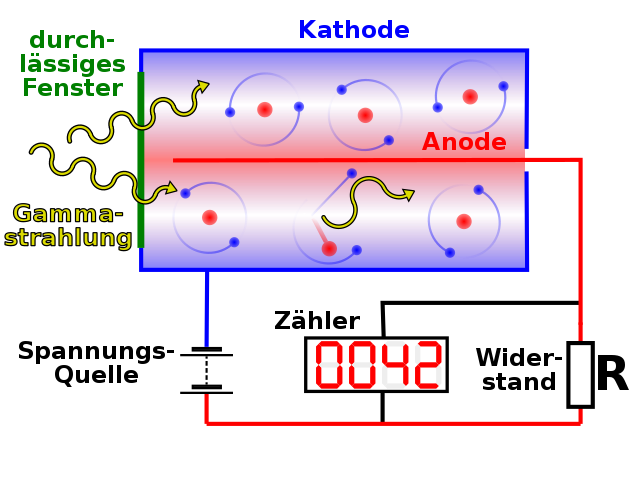
\includegraphics[width=0.7\textwidth]{../media/B3.1/640px-Geiger_Mueller_Counter_with_Circuit-de.svg.png}
	\caption{Aufbau eines typischen Geiger--Müller--Zählrohrs \cite{File:Geigerzählrohr}}
	\label{fig:Geiger--Müller--Zählrohr}
\end{figure}

\subsubsection{Totzeit}
\label{Totzeit}
Ganz allgemein beschreibt Totzeit $\tau$ die Zeit, die nach der Registrierung eines Ereignisses durch einen Detektor verstreicht, bis der Detektor wieder messbereit ist. \cite{Totzeit}

Wie schon beschrieben ist während der Totzeit $\tau$ keine Strahlungsmessung möglich. Dadurch weicht die gemessene Zählrate $a^\prime$ von der tatsächlichen Rate $a$ ab. Um die tatsächliche Rate zu bestimmen, muss für jedes gemessene Teilchen die Anzahl der Detektionen in der Totzeit $a\tau$ addiert werden. Dies beschreibt die tatsächlich geschehenen Ereignisse, die während der Totzeit nicht gemessen werden können.

Analog kann der gemessene Mittelwert $m^\prime$ von in einem Zeitraum $T$ gemessenen Ereignissen korrigiert werden, um den korrigierten Mittelwert $m=aT$ zu erhalten. Dieser ist größer als der gemessene Mittelwert.

\begin{eqnarray}
	a &=& a^\prime \cdot(1 + a\tau) \\
	\Leftrightarrow\quad a &=& \frac{a^\prime}{1-a^\prime\tau} \label{eq:Totzeitkorrigiert Rate}\\
	m &=&\frac{m'}{1-a'\tau} \label{eq:Totzeitkorrigiert EW}
\end{eqnarray}

\noindent
Das Verhältnis von Varianz $\sigma^2$ und Mittelwert $m$ der gemessenen Verteilung entspricht der tatsächlichen Verteilung. Weisen die Messwerte eine Poissonverteilung auf, dann sind Varianz $\sigma^2$ der Messung mit dem Mittelwert $m$ identisch.

\begin{eqnarray}
	\frac{\sigma}{m}&=&\frac{\sigma^\prime}{m^\prime}\\
	\Rightarrow\quad \sigma^{\prime\,2} & = &\frac{m^{\prime\,2}}{m} \\
		%&=& m^\prime\cdot\frac{a^\prime}{a} \\
		&=& m^\prime\cdot(1-a^\prime\tau) \\
	\sigma^2
		%&=& \sigma^{\prime\,2}\left(\frac{a}{a^\prime}\right)^2\\
		&=& \frac{m^\prime}{1-a\tau}
\end{eqnarray}

\noindent
Hierbei wurden die Verhältnisse $\frac{\sigma}{m}$ und $\frac{a^\prime}{a}$ durch die Gleichungen \eqref{eq:Poisson STD/EW} und \eqref{eq:Totzeitkorrigiert EW} beschrieben.

\hypertarget{einfluss-der-totzeit}{%
\subsubsection{Totzeit im $\chi^2$--Test}\label{einfluss-der-totzeit}}

Die Totzeit der Länge $\tau$ hat einen Einfluss auf die gemessenen Zählraten. Anstatt einer Zählrate von $\frac{n_i}{\Delta t}$ wird eine totzeitkorrigierte Anzahl $k_i$ gemessen. Dadurch kann ein korrigierter Mittelwert $M$ nach $\eqref{mittlereRate}$ bestimmt werden und man erhält eine korrigierte Abweichung $\chi^2_\mathrm{korr}$. Die korrigierte Rate wird nach Gleichung \eqref{eq:Totzeitkorrigiert Rate} bestimmt.

\begin{eqnarray}
    k_i &=&
        \frac{
            n_i
        }{
            1 - \frac{m}{\Delta t}\tau
        } \label{korrRate} \\
    M &=& \sum_{i=1}^N \frac{k_i}{N} \label{korrAVG} \\
    \chi^2_\mathrm{korr} &=& \sum_{i=1}^N
        \frac{(k_i - M)^2}{M} \label{ChiKorrDef}
\end{eqnarray}

\noindent
Durch Einsetzen der Gleichungen $\eqref{korrRate}$-$\eqref{korrAVG}$ sowie $\eqref{ChiSquared}$ kann man $\eqref{ChiKorrDef}$ vereinfachen und man erhält die folgende vereinfachte Relation. Hier sieht man, dass die korrigierte Abweichung $\chi^2_\mathrm{korr}$ kleiner als die nicht--korrigierte Abweichung $\chi^2$ ist, was kontraintuitiv wahrgenommen werden kann.

\begin{eqnarray}
    \chi^2_\mathrm{korr} &=&
        \frac{1}{1 - \frac{m}{\Delta t}\tau} \cdot \chi^2
\end{eqnarray}

\subsubsection{Zwei--Präparate--Methode}
Die Zwei--Präparate--Methode wird verwendet, um die Totzeit zu messen. Man misst die Zählrate von zwei verschiedenen Präparaten $z^\prime_{1/2}$ jeweils einzeln und dann von beiden zusammen $z^\prime_{12}$. Zusätzlich wird die Untergrundzählrate $z^\prime_0$ ohne Präparate gemessen.

Somit erhält man gemessene Werte $z^\prime_i$ und sowie wahre Werte $z_i$. Die wahren Zählraten $z_i$ sind durch die Präparate und den Untergrund entstanden.

Nun seien $p_{1,\,2,\,12}$ die Zählraten, die sich durch die Verwendung von Präparaten ergeben. Daraus erhält man ein lösbares Gleichungssystem mit von je acht Gleichungen und Unbekannten.  Die letzten Gleichungen ergeben sich durch die Totzeitkorrektur \eqref{eq:Totzeitkorrigiert Rate} der Zählraten.

%\begin{eqnarray}
%	z_1 &=& p_1+u \\
%	z_2 &=& p_2+u \\
%	z_{12} &=& p_{12}+u \\
%	z_1 &=& \frac{z^\prime_1}{1-z^\prime_1 \tau} \\
%	z_2 &=& \frac{z^\prime_2}{1-z^\prime_2 \tau} \\
%	z_{12} &=& \frac{z^\prime_{12}}{1-z^\prime_{12} \tau} \\
%	u &=&\frac{u^\prime}{1-u^\prime\tau} \\
%	p_{12} &=& p_1+p_2
%\end{eqnarray}
\begin{eqnarray}
	p_{12} &=& p_1 + p_2 \\
	\forall i\in\{1,\,2,\,12\}:\qquad
		z_i &=& p_i + z_0 \\
	\forall i\in\{0,\,1,\,2,\,12\}:\quad
		z_i &=& \frac{z^\prime_i}{1-z^\prime_i \tau}
\end{eqnarray}

\noindent
Die Lösung dieses Gleichungssystems ergibt die Totzeit. Diese Formel wird auch als \emph{Mitternachtsformel} bezeichnet

\begin{align}
	\tau _{1,\,2} \eqspaced& \frac{-B \pm \sqrt{B^2 - 4AC}}{2A} \label{eq:Totzeit Mitternachtsformel} \\
	\begin{split}
		A \eqspaced& u'z'_{12}z'_2 - z'_1z'_12z'_2 + u'z'_{12}z'_1 - u'z'_1z'_2 \\
		B \eqspaced& -2z'_{12}u' + 2z'_1z'_2 \\
		C \eqspaced& z^\prime _{12} - z^\prime _1 + u^\prime  - z^\prime _2
	\end{split}
\end{align}

\clearpage
\hypertarget{durchfuxfchrung}{%
\section{Durchführung}\label{durchfuxfchrung}}
\subsection{Versuchsaufbau}
Der Aufbau beinhaltet zwei $\ce{^{137}Cs}$--Quellen und Zählrohr mit angeschlossener Elektronik. Die am Zählrohr angeschlossene Spannung lässt sich variieren, die Zählrohrelektronik erzeugt ein Rechtecksignal je detektiertem Ereignis. Dieses Signal wird an einen Zähler und an einen Computer übertragen. Auf dem Computer können die Ereignisse zeitaufgelöst gemessen werden.

Zur Bearbeitung der Daten sind am Computer drei Python-Programme vorinstalliert, mit denen die Messdaten verarbeitet werden können. Mit \code{divide.py} Ereignisse in Zeitintervallen fester Größe, z.B.  jeweils $10\mathrm{\,s}$, gezählt. Mittels \code{binomial.py} kann eine Binomialverteilung aus den Daten extrahiert werden, mit \code{interval.py} eine Intervallverteilung.

\subsection{Messungen}
Es wurden $3$ lange und $12$ kurze Messungen durchgeführt.

Bei den ersten beiden langen Messungen wurde nur Probe $A$ verwendet, bei der dritten langen Messung die Probe $A$ und $B$. Eine Einzelmessung von Probe $A$ und die gemeinsame Messung wurden bei einer Spannung von $500\mathrm{\,V}$ durchgeführt, die zweite Einzelmessung bei $600\mathrm{\,V}$. Hierbei wurden die Ereignisse zeitaufgelöst gemessen.

Die $12$ kurzen Messung dienten der Bestimmung der Totzeit mit der Zwei--Präparate--Methode. Hierzu wurden jeweils bei Spannungen von $500\mathrm{\,V}$, $550\mathrm{\,V}$ und $600\mathrm{\,V}$ die Ereignisse in jeweils $5\mathrm{\,min}$ gemessen. Dabei wurden die Proben $A$ und $B$ sowohl einzeln als auch gemeinsam verwendet. Die letzten drei kurzen Messungen erfolgten ohne Proben, um den Untergrund zu vermessen.

\clearpage
\hypertarget{auswertung}{%
\section{Auswertung}\label{auswertung}}

\hypertarget{poissonverteilung}{%
\subsection{Poissonverteilung}\label{poissonverteilung}}
Als erstes wird der Zerfall der Proben mit der Poisson--Verteilung verglichen. Dazu werden die Messergebnisse jeweils mit einer dazu passenden Poisson--Verteilung aufgetragen, was in Abbildung \ref{fig:poisson single} dargestellt ist.

Der Mittelwert und die Varianz der jeweiligen Poisson--Verteilungen sind als $\lambda$ gegeben und in Tabelle \ref{table:poisson} dargestellt.

\begin{eqnarray}
	P(n,\lambda) = N \cdot \frac{\lambda^n e^{-\lambda}}{n!}
\end{eqnarray}

\begin{table}[h!]
	\centering
	\begin{tabular}{c|c|c}
		Probe & Spannung $[\mathrm{V}]$ & $\lambda$ \\
		\hline
		$A$ & $500$ & $7.1$ \\
		$A$ & $600$ & $8.5$ \\
		$A+B$ & $500$ & $13.5$ \\
	\end{tabular}
	\caption{Mittelwerte bzw. Varianzen $\lambda$  der drei Poisson--Verteilungen}
	\label{table:poisson}
\end{table}

\begin{figure}
	\centering
	\begin{minipage}{0.49\textwidth}
		\centering
		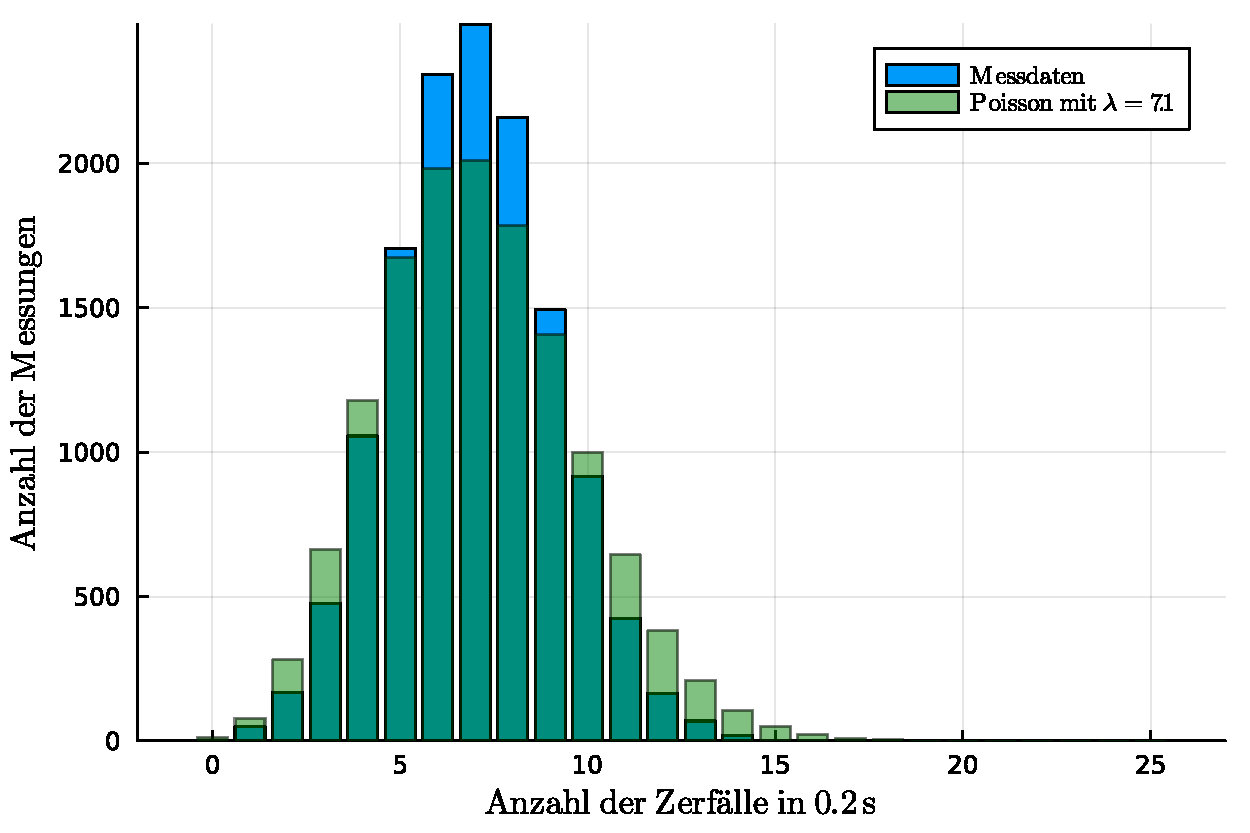
\includegraphics[width=\textwidth]{../media/B3.1/poisson1.pdf}
		\caption*{Probe $A$, $500 \mathrm{\, V}$}
	\end{minipage}
	\begin{minipage}{0.49\textwidth}
		\centering
		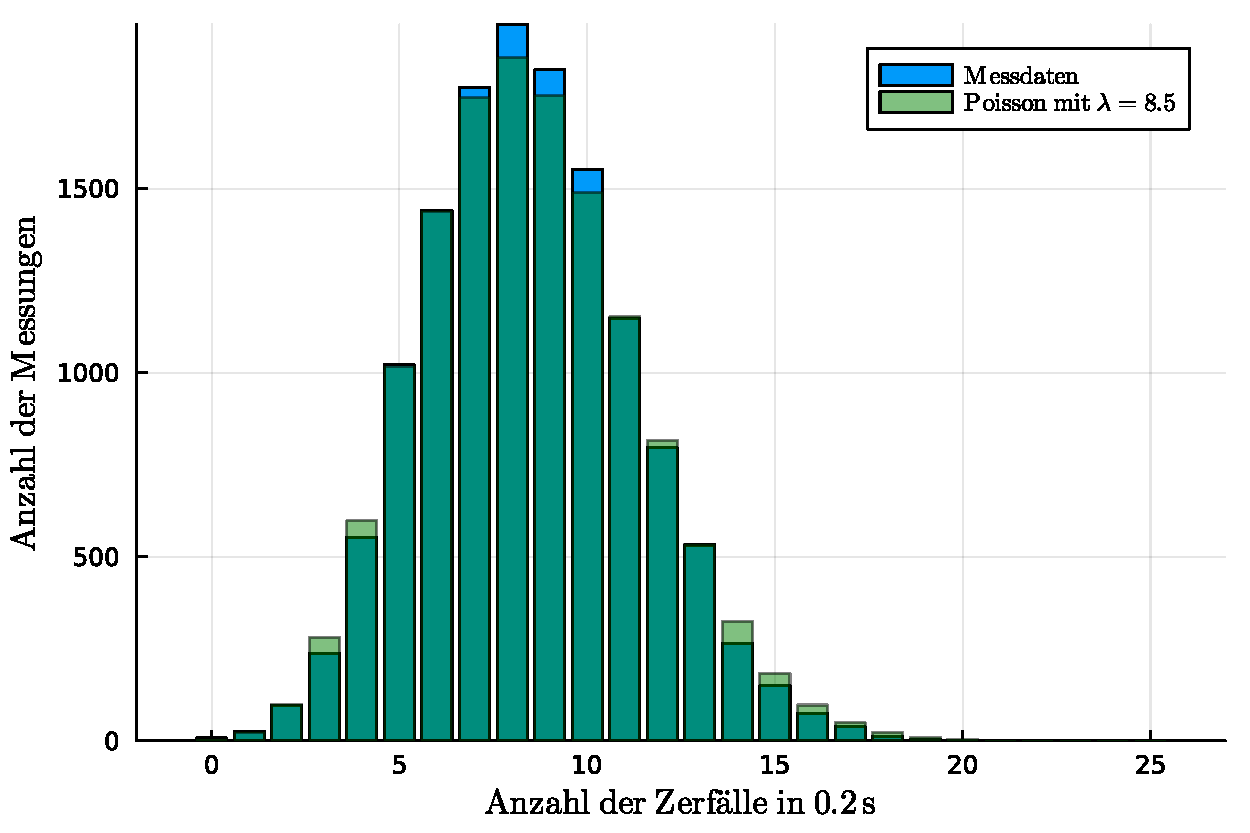
\includegraphics[width=\textwidth]{../media/B3.1/poisson2.pdf}
		\caption*{Probe $A$, $600 \mathrm{\, V}$}
	\end{minipage}
	\vspace{3pt}

	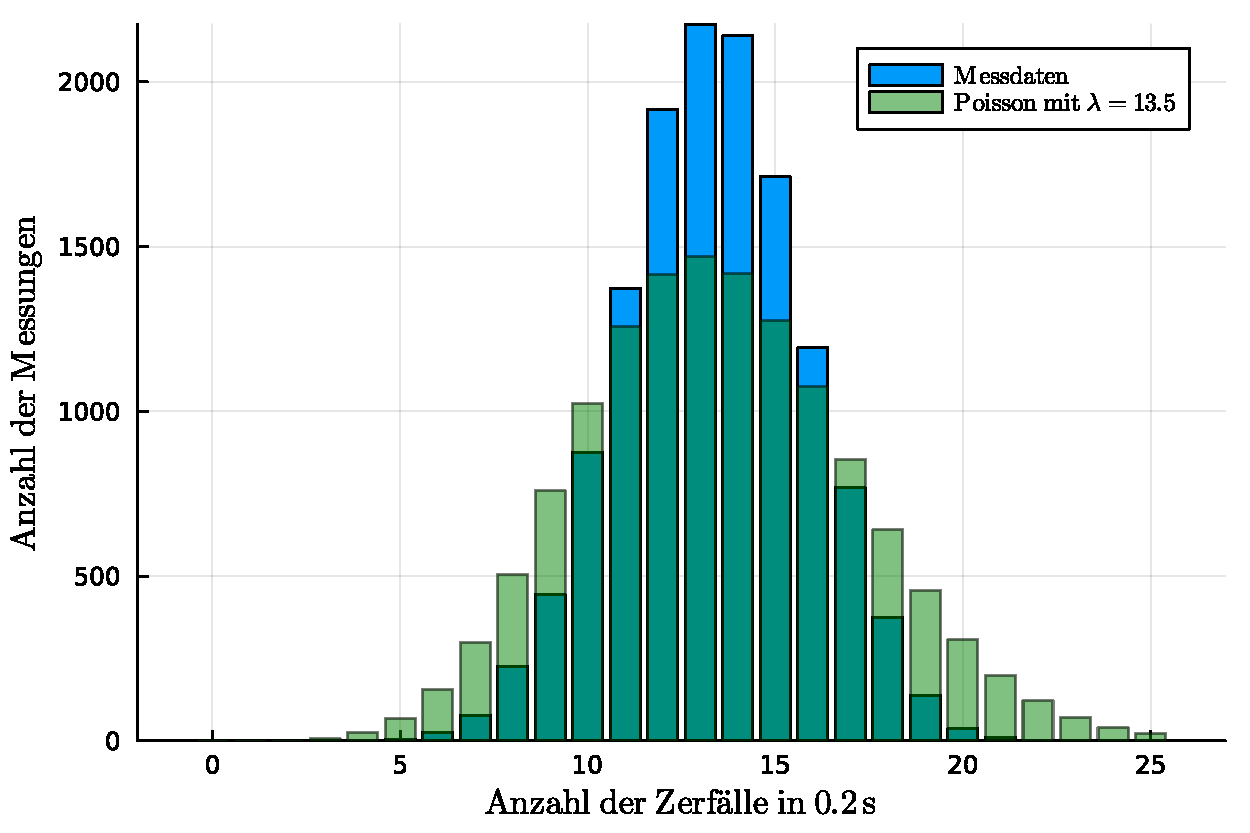
\includegraphics[width=0.49\textwidth]{../media/B3.1/poisson3.pdf}
	\caption*{Proben $A$ und $B$ gemeinsam, $500 \mathrm{\, V}$}
	\vspace{3pt}
	
	\caption{Messwerte und Poisson--Verteilungen}
	\label{fig:poisson single}
	\vspace{12pt}
	
	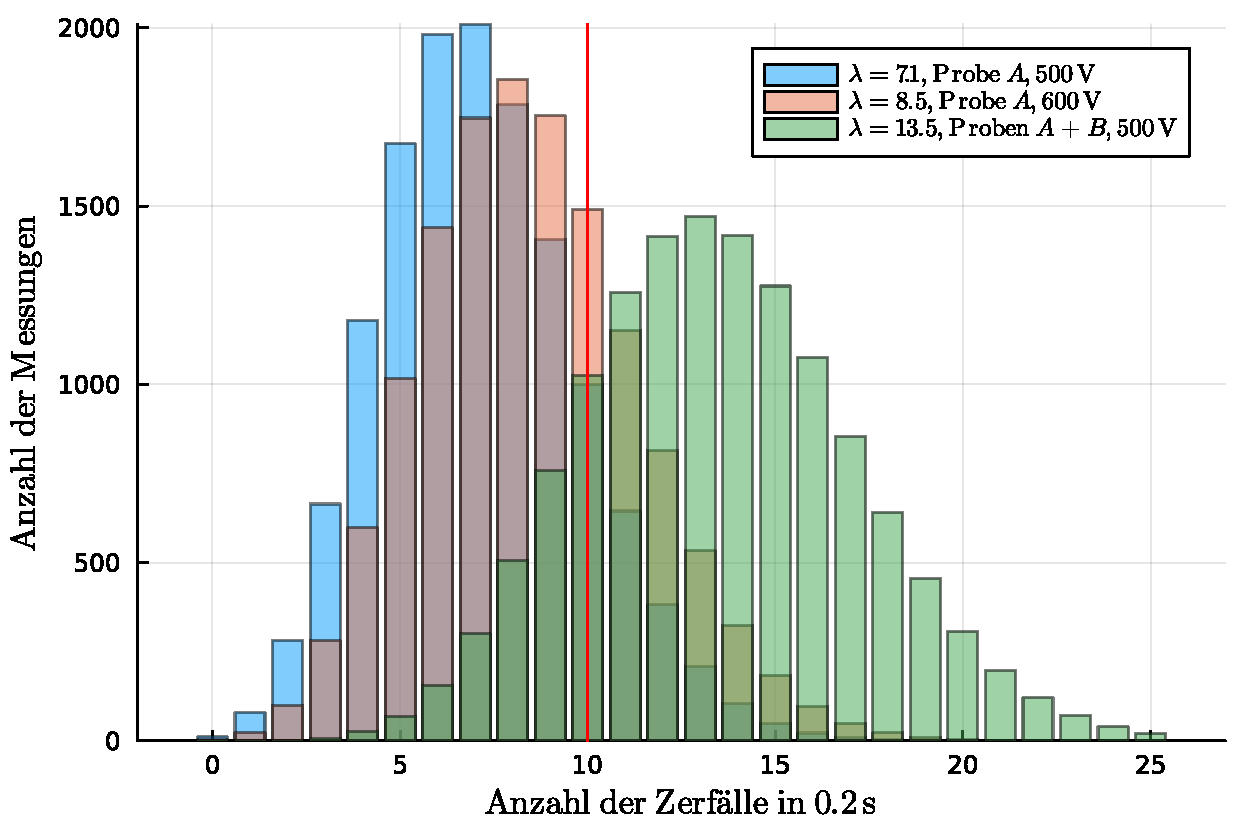
\includegraphics[width=0.7\textwidth]{../media/B3.1/allePoisson.pdf}
	\caption{Alle drei Poisson--Verteilungen zusammen\\
		Die Grenze der Faustregel für den Mittelwert einer sinnvolle Poisson--Annäherung ist in rot markiert}
	\label{fig:allePoisson}	
\end{figure}

\noindent
Dabei wurde die Anzahl an Zerfällen innerhalb von relativ kurzen Zeitintervallen von $0.2 \mathrm{\,s}$ jeweils in einem Balken dargestellt. Die kurzen Zeitintervalle sorgen dafür, dass der Mittelwert der Messdaten klein bleibt und so eine Poisson--Verteilung nach der in Abschnitt \ref{Poissonverteilung} erwähnten Faustregel eine sinnvolle Näherung ergibt, solange für den Mittelwert gilt $\lambda \leq 10$.

Für die Messungen  Probe $A$ folgen die Messwerte recht genau der Poisson--Verteilung, die gemeinsame Messung der Proben $A$ und $B$ zeigt allerdings deutlichere Unterschiede auf. Die Poisson--Verteilung ist dort deutlich breiter als die Messwerte und um den Mittelwert herum nicht so hoch. Hier bestätigt sich die besprochene Faustregel, dass die Poisson--Verteilung für $\lambda > 10$ keine gute Näherung mehr darstellt und stattdessen eher die Gaußverteilung verwendet werden sollte.

Alle drei Poisson--Verteilungen sind nochmal gemeinsam in Abbildung \ref{fig:allePoisson} dargestellt. Es ist ersichtlich, dass der Mittelwert der Verteilung sowohl bei höheren Spannungen, als auch bei mehr Probenmaterial steigen. Außerdem werden die Verteilungen breiter und flacher, je größer der Mittelwert ist.

Allerdings sind alle drei theoretischen Verteilungen etwa breiter als die Messdaten. Dies ist besonders gut bei der ersten und dritten Messung zu sehen. Dies ist durch die Totzeit erklärt, die Mittelwert und Standardabweichung der Messung verringert.\footnote{Vergleiche Abschnitt \ref{Totzeit}}

\newpage
\hypertarget{gauuxdfverteilung}{%
\subsection{Gaußverteilung}\label{gauuxdfverteilung}}
Für größere Mittelwerte ist der Vergleich mit der Gaußverteilung sinnvoll. Dazu werden die Messewerte für Zeitintervalle von $5 \mathrm{\,s}$ zusammengefasst.

Weiterhin wird ein sogenanntes \textit{Binning} von $8$ verwendet. Dies bedeutet, es werden $8$ benachbarte Balken zu einem zusammengefasst. Der erste Balken gibt also demnach an, wie oft innerhalb von $5 \mathrm{\, s}$ zwischen $0$ und $7$ Zerfälle detektiert wurden. Dies ist in Abbildung \ref{fig:gauss single} dargestellt.

Dazu ist jeweils die theoretische Gaußkurve eingezeichnet, die sich völlig aus den gemessenen Werten ergibt. Der Mittelwert $m$ der $n$ Messungen wird aus der gemessenen Zählrate $z^\prime$ gebildet, die in Tabelle \ref{table:zählraten gauss} dargestellt sind. $F$ ist ein Normierungsfaktor, der sich aus der Summe der Höhen aller Balken ergibt.

Die Messwerte sowie die Mittelwerte der Gaußkurven sind in Tabelle \ref{table:zählraten gauss} angegeben.

\begin{eqnarray}
	P(x) &=& \frac{1}{\sqrt{2 \pi m}} \cdot F \cdot \sqrt{n} \cdot e^{- \frac{(x-m)^2}{2m/n}} \\
	m &=& z^\prime \cdot \frac{\Delta t}{n}
\end{eqnarray}

\begin{table}[h!]
	\centering
	\begin{tabular}{c|c|c|c|c}
		Probe
			& Spannung $[\mathrm V]$
			& Zerfälle $[(300 \mathrm{\, s})^{-1}]$
			& Zählrate $z^\prime$ $[\mathrm{ms^{-1}}]$ &
			Mittelwert $m$ $[\mathrm{ms^{-1}}]$\\
		\hline
		$A$ & $500$ & $11044$ & $36.80$ & $23.01$ \\
		$A$ & $600$ & $12917$ & $43.06$ & $26.90$ \\
		$A+B$ & $500$ & $20300$ & $67.70$ & $42.29$ \\
	\end{tabular}
	\caption{Zählraten der Quellen bei unterschiedlichen Spannungen}
	\label{table:zählraten gauss}
\end{table}
\begin{figure}[h!]
	\centering
	\begin{minipage}{0.3\textwidth}
		\centering
		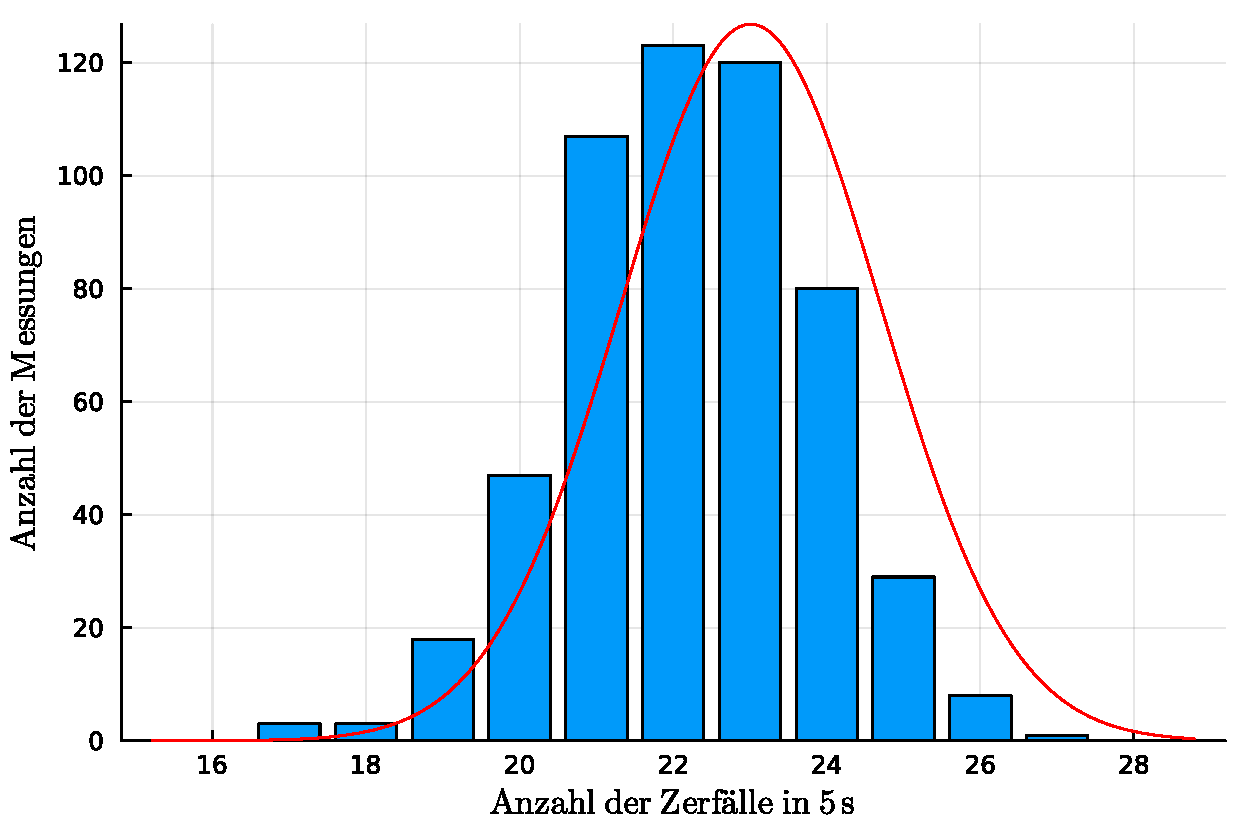
\includegraphics[width=\textwidth]{../media/B3.1/gauss1.pdf}
		\caption*{Probe $A$, $500 \mathrm{\, V}$,\\Binning $8$}
	\end{minipage}
	\begin{minipage}{0.3\textwidth}
		\centering
		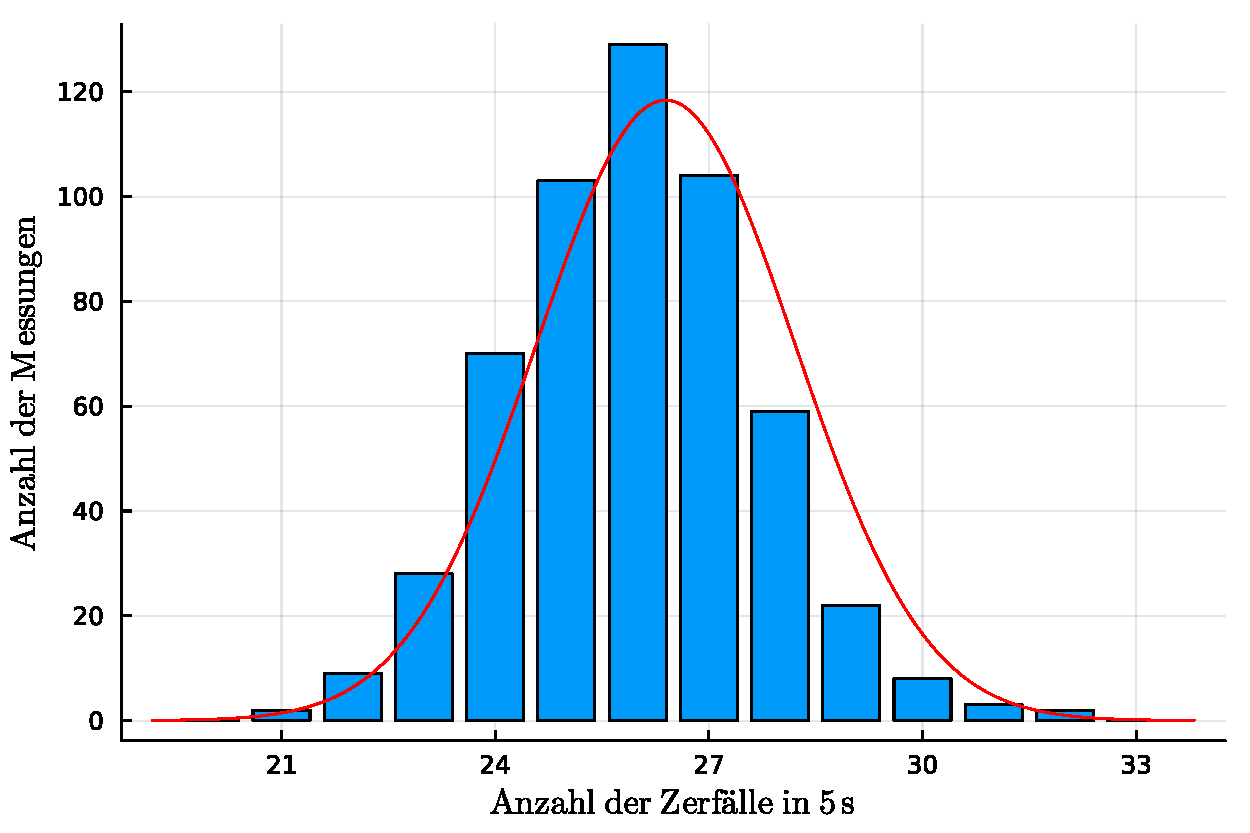
\includegraphics[width=\textwidth]{../media/B3.1/gauss2.pdf}
		\caption*{Probe $A$, $600 \mathrm{\, V}$,\\Binning $8$}
	\end{minipage}
	\begin{minipage}{0.3\textwidth}
		\centering
		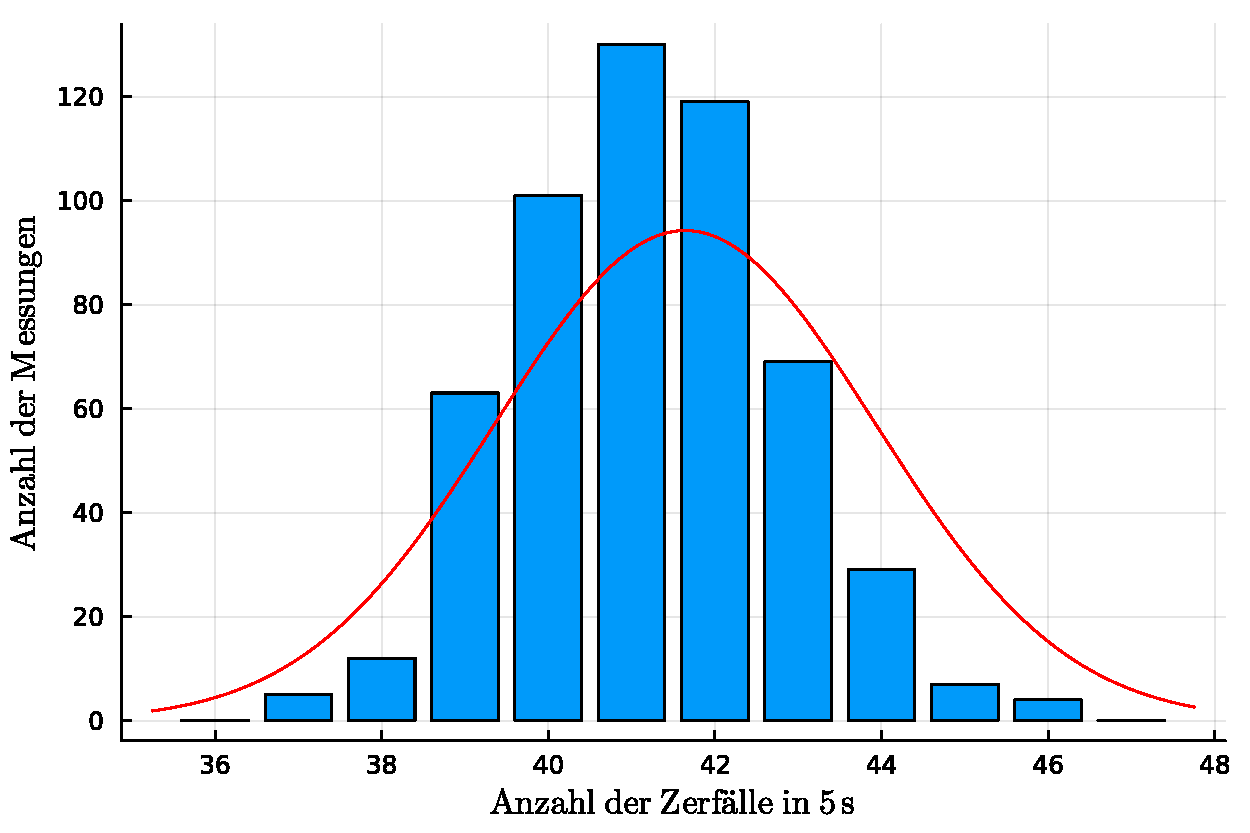
\includegraphics[width=\textwidth]{../media/B3.1/gauss3.pdf}
		\caption*{Proben $A$ und $B$,\\$500 \mathrm{\, V}$, Binning $8$}
	\end{minipage}
	\vspace{3pt}
	
	\vspace{3pt}
	
	\caption{Messwerte und Gauß--Verteilungen}
	\label{fig:gauss single}
	\vspace{12pt}
\end{figure}

\noindent
Alle Gauß--Verteilungen passen gut zu den Messungen. Bei der $500\mathrm{\,V}$--Messung von Probe $A$ ist die Gauß--Kurve etwas weiter rechts als die Messwerte. Dies ist durch die Verschiebung des Mittelwerts durch die Totzeit begründet.

Bei der anderen Messung von Probe $A$ ist der Peak der Kurve ein wenig zu höher, bei der gemeinsamen Messung der Proben $A$ und $B$ ist dies noch stärker der Fall. Zudem kann man bei letzterem Vergleich sehen, dass die gemessene Verteilung schmaler ist als die Gauß--Verteilung. Beides kann wiederum durch die Totzeit erklärt werden. Diese verringert anscheinend nicht nur die Position des Mittelwerts, sondern auch die Standardabweichung der Messung.

Bei der Poisson--Verteilung ist dies einfach zu begründen.\footnote{Vergleiche Abschnitt \ref{Totzeit}} Es lässt sich vermuten, dass die Totzeit bei der Gauß--Verteilung ähnlich wie bei der Poisson--Verteilung zutrifft.

\hypertarget{intervallverteilung}{%
\subsection{Intervallverteilung}\label{intervallverteilung}}
In Abbildung \ref{fig:interval} sind die gemessenen Intervall--Verteilungen für die Messung von Probe $A$ bei $500 \mathrm{\, V}$ für $n = 0,1,2$ aufgetragen.

\begin{figure}[h]
	\centering
	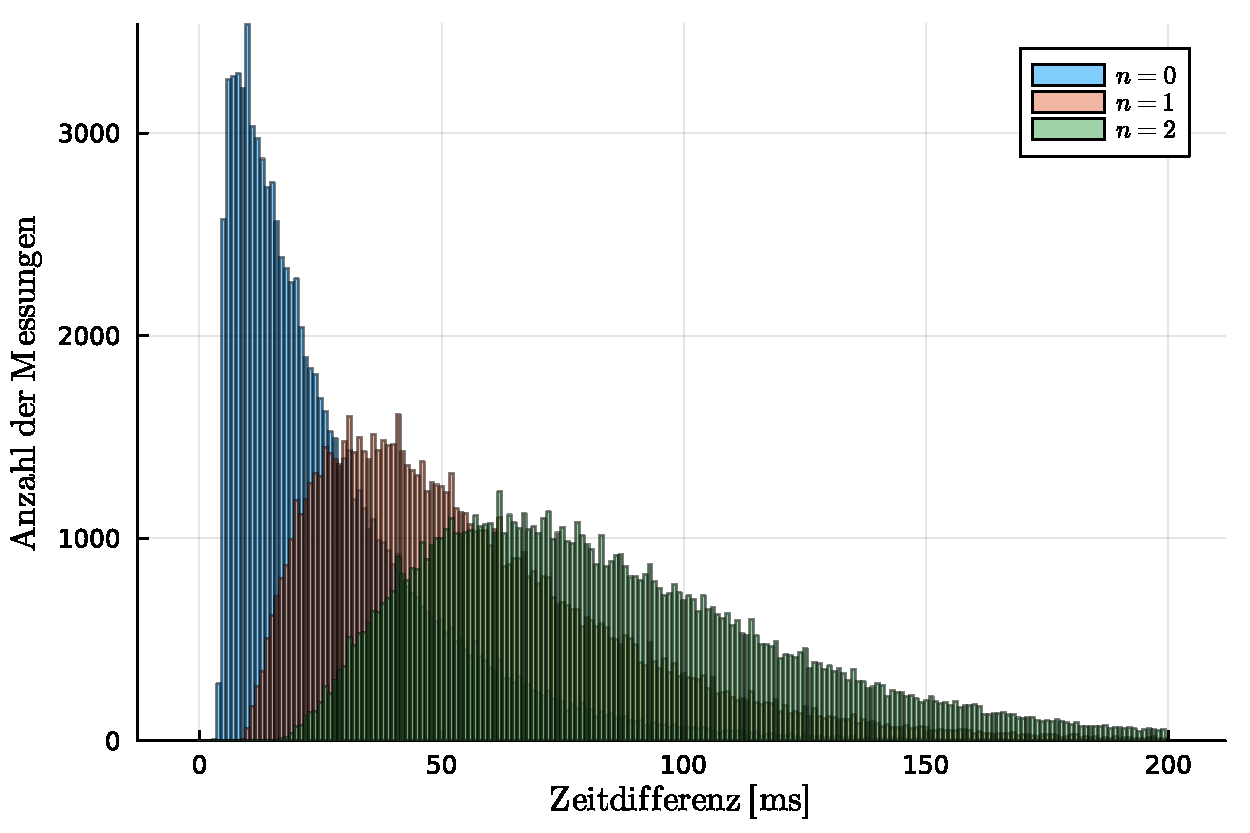
\includegraphics[width=0.7\textwidth]{../media/B3.1/interval.pdf}
	\caption{Gemessene Intervall--Verteilungen für Probe $A$ bei $500 \mathrm{\, V}$ für $n = 0,1,2$}
	\label{fig:interval}
\end{figure}

Die gemessene Intervall--Verteilung mit $n = 0$ wird nun mit der theoretischen Verteilung verglichen. Dafür wird die theoretische Intervall--Verteilung $P_0$ an die Messwerte gefittet, die durch Gleichung \eqref{eq:Intervallverteilung} beschrieben ist. Daber wurde der Fitting--Parameter $a = 4.3 \cdot 10^{-2} \mathrm{\,ms^{-1}}$ ermittelt. Zudem wurde die Normierungskonstante $N(a)=T\cdot a$ verwendet, die von $a$ und der Messdauer $T=45\mathrm{\,min}$ in Sekunden.

\begin{eqnarray}
	P(t) &=& N(a) \cdot a \cdot e^{-at} \\
	N &=& T \cdot a
\end{eqnarray}

\noindent
Das Ergebnis ist in Abbildung \ref{fig:intervalFit} zu sehen. Dabei ist zu beachten, dass die ersten acht Messwerte der gemessenen Intervall--Verteilung für den Fit ausgeschlossen wurden, da sie in einem Zeitabschnitt liegen, der kleiner als die erwartete Totzeit ist, wodurch ihre Ergebnisse stark von den erwarteten abweichen dürften.

\begin{figure}
	\centering
	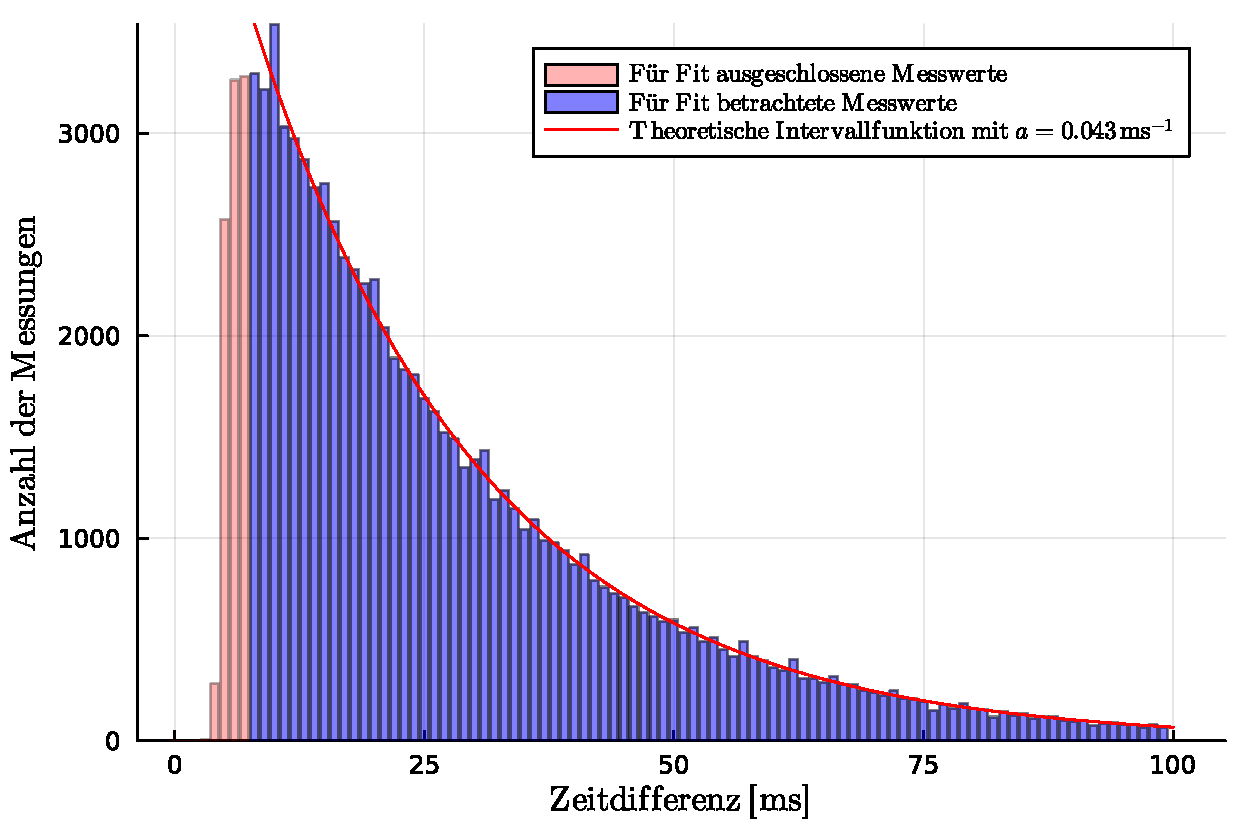
\includegraphics[width=0.7\textwidth]{../media/B3.1/intervalFit.pdf}
	\caption{Gemessene Intervall-Verteilung für Quelle Nr. 6 bei $500 \mathrm{\, V}$ für $n = 0$ und dazu gefittete theoretische Intervall-Verteilung}
	\label{fig:intervalFit}
\end{figure}

Aus dem so bestimmten Fit-Parameter $a$ lässt sich nun mittels Gleichung \eqref{eq:Totzeitkorrigiert Rate} die Totzeit $\tau$ ermitteln.

\begin{eqnarray}
	\tau &=& \frac{1}{a'} - \frac{1}{a}
\end{eqnarray}

\noindent
Dabei ist $a' \approx 36.80 \cdot 10^{-2} \mathrm{\,ms^{-1}}$ die für diese Quelle gemessene Zählrate aus Tabelle \ref{table:zählraten gauss}. Dadurch ergibt sich für die Totzeit $\tau \approx 3.9 \mathrm{\, ms}$.

Für die anderen beiden gemessenen Intervall--Verteilungen für $n = 1,2$ ist ein Fit--Versuch mit der theoretischen Kurve nicht sinnvoll. Dies liegt daran, dass die Totzeit bei $n = 1,2$ nicht nur im vordersten Teil der Verteilung sichtbar ist, wie bei $n = 0$. Bei ihnen verändert die Totzeit hingegen die ganze Verteilung, wodurch kein sinnvoll zu fittender Bereich mehr übrig bleibt. Dem ist so, weil die Messung des dritten Zerfalls ebenfalls einer Totzeit unterliegt. Wann der zweite Zerfall allerdings gemessen wurde, ist aus den Daten nicht ersichtlich und vor allem immer unterschiedlich, wodurch an immer anderen Stellen eine Veränderung durch die Totzeit hinzukommt.

\hypertarget{Totzeit bestimmen}{\subsection{Totzeit}\label{Totzeit bestimmen}}
Die Totzeit $\tau$ wird hier mit der Zwei--Präparate--Methode bestimmt. Es wurden für die Proben $A$ und $B$ jeweils $N_A$ bzw. $N_B$ Ereignisse gemessen. Weiterhin wurden $N_{AB}$ Ereignisse bei Verwendung beider Proben $A$ und $B$ sowie $N_0$ Ereignisse ohne Proben gemessen. Letztere wurden durch die Untergrundstrahlung verursacht.

Aus den Zählungen $N_i$ und der Dauer der Messungen $T=5\mathrm{\,min}$ lassen sich Zählraten $n_i$ ermitteln. Die Ergebnisse sind in den Tabellen \ref{tab:Totzeit Ereignisse} dargestellt. Der Fehler der Zählungen $\Delta N_i$ wird durch die statistische Ungenauigkeit gegeben.

Aus diesen Zählraten $z_i$ kann die Totzeit $\tau_{1,2}$ mit der Mitternachtsformel \eqref{eq:Totzeit Mitternachtsformel} ermittelt werden. Die Ungenauigkeiten  $\Delta \tau_{1/2}$ sowie $\Delta A$, $\Delta B$, $\Delta C$ werden durch Gauß'sche Fehlerfortpflanzung ermittelt. Diese Ergebnisse sind in Tabelle \ref{tab:Totzeiten} dargestellt. Hierbei fällt der sehr hohe relative Fehler für die Totzeiten auf.

\begin{eqnarray}
	\Delta N &=& \sqrt{N} \\
	n_i &=& \frac{N_i}{T} \\
	\Delta n_i &=& \frac{\Delta N_i}{T}
\end{eqnarray}

\begin{table}[h!]
	\centering
	\begin{tabular}[h]{c|c|c|c|c}
		Spannung $[\mathrm V]$
			& $N_A\equiv N_1$
			& $N_B\equiv N_2$
			& $N_{AB}\equiv N_{12}$
			& $N_0$ \\
		\hline
		$500$ & $11044$ & $15833$ & $20300$ & $2396$ \\
		$550$ & $12260$ & $17914$ & $25509$ & $2513$ \\
		$600$ & $12917$ & $19421$ & $28522$ & $2550$ \\
	\end{tabular}
	\caption{Gemessene Ereignisse}
	\label{tab:Totzeit Ereignisse}
	\vspace{12pt}

	\begin{tabular}[h]{c|c|c|c|c|c}
		Spannung $[\mathrm V]$
			& $z_1$ $[\mathrm s^{-1}]$
			& $z_2$ $[\mathrm s^{-1}]$
			& $z_{12}$ $[\mathrm s^{-1}]$
			%& $z_0$ $[\mathrm s^{-1}]$
			& $\tau_1$ $[\mathrm{ms}]$
			& $\tau_2$ $[\mathrm{ms}]$ \\
		\hline
		$500$
			& $37 \pm 6$
			& $53 \pm 7$
			& $68 \pm \ 8$
			%& $7.9 \pm 2.8$
			& $6 \pm 9$ $(\pm\, 147\,\%)$
			& $22 \pm 18$ $(\pm\, 84\,\%)$ \\
		$550$
			& $41 \pm 6$
			& $60 \pm 8$
			& $85 \pm \ 9$
			%& $8.0 \pm 3.0$
			 & $2 \pm 5$ $(\pm\, 223\,\%)$
			 & $20 \pm 12$ $(\pm\, 59\,\%)$ \\
		$600$
			& $43 \pm 7$
			& $65 \pm 8$
			& $95 \pm 10$
			%& $8.5 \pm 3.0$
			& $1 \pm 4$ $(\pm\, 368\,\%)$
			& $19 \pm 10$ $(\pm\, 51\,\%)$ \\
	\end{tabular}
	\caption{Ermittelte Zählraten $z_i$ und Totzeiten $\tau_i$}
	\label{tab:Totzeiten}
\end{table}

\noindent
Die Werte von $\tau_1$ stimmen eher als die von $\tau_2$ mit den Totzeiten aus der Intervallverteilung überein. $\tau_2(500\mathrm{\,V})$ trifft innerhalb der Fehlergrenzen ebenfalls diesen Wert, die zwei anderen allerdings nicht mehr.

\begin{align}
	\begin{split}
		(\Delta \tau _1)^2\eqspaced
		&
			\left(
				\left(
					\frac{-B-\sqrt{B^2 - 4AC}}{2A^2}
					- \frac{C}{A\sqrt{B^2 - 4AC}}
				\right) \Delta A
			\right) ^2 \\
		&
				+\left(
					\frac{1}{2A}\left(
						\frac{B}{\sqrt{B^2 - 4AC}} - 1
					\right) \Delta B
				\right)^2
				+ \left(
					-\frac{\Delta C}{\sqrt{B^2 - 4AC}}
				\right)^2
	\end{split}\\
	\begin{split}
		(\Delta \tau _1)^2\eqspaced
			&
				\left(
					\left(
						\frac{\sqrt{B^2 - 4AC}+B}{2A^2}
						+ \frac{C}{A\sqrt{B^2 - 4AC}}
					\right) \Delta A
				\right)^2\\
			&
				+ \left(
					\frac{1}{2A}\left(
						\frac{-B}{\sqrt{B^2 - 4AC}} - 1
					\right) \Delta B
				\right)^2
				+ \left(
					\frac{\Delta C}{\sqrt{B^2 - 4AC}}
				\right) ^2
	\end{split}
\end{align}

\begin{align}
	\begin{split}
		(\Delta A)^2 \eqspaced
		& \big((-z^\prime _{12}z^\prime _2 + u^\prime z^\prime _{12} - u^\prime z^\prime _2)\Delta z^\prime _1\big)^2
			+\big((u^\prime z^\prime _{12}-z^\prime _1z^\prime _{12}-u^\prime z^\prime _1)\Delta z_2\big)^2 \\
		&+\big((u^\prime z^\prime _2-z^\prime _1z^\prime _2+u^\prime z^\prime _1)\Delta z^\prime _{12}\big)^2
			+ \big((z^\prime _{12}z^\prime _2 + z^\prime _{12}z^\prime _1 -z^\prime _1z^\prime _2)\Delta u^\prime \big)^2
	\end{split} \\
	(\Delta B)^2 \eqspaced&  (2z^\prime _2 \Delta z^\prime _1)^2 + (2z^\prime _1 \Delta z^\prime _2)^2 + (-2u^\prime  \Delta z^\prime _{12})^2 + (-2z^\prime _{12} \Delta u^\prime )^2 \\
	(\Delta C)^2 \eqspaced& (\Delta z^\prime _1)^2 + (\Delta z^\prime _2)^2 + (\Delta z^\prime _{12})^2 + (\Delta u^\prime )^2
\end{align}

\noindent
Zusätzlich wurde die Totzeit digital ermittelt, dazu wurde das Paket \code{Measurements} in der Programmiersprache \code{Julia} verwendet. \cite{Julia:Measurements} Die Ergebnisse für $\tau _{1,2}$ sind gleich geblieben, allerdings unterscheiden sich die ermittelten Fehler, zum Teil erheblich. Die Ergebnisse sind in Tabelle \ref{tab:Totzeit m. Julia} dargestellt.

\begin{table}[h!]
	\centering
	\begin{tabular}[h]{c|c|c}
		Spannung $[\mathrm V]$
			& $\tau_1$ $[\mathrm{ms}]$
			& $\tau_2$ $[\mathrm{ms}]$ \\
		\hline
		$500$ & $6 \pm 6$ $(\pm\, 89\,\%)$ & $22.0 \pm 2.6$ $(\pm\, 12\,\%)$  \\
		$550$ & $2 \pm 4$ $(\pm\, 190\,\%)$ & $19.8 \pm 2.1$ $(\pm\, 11\,\%)$ \\
		$600$ & $1 \pm 4$ $(\pm\, 340\,\%)$ & $18.5 \pm 1.9$ $(\pm\, 10\,\%)$ \\
	\end{tabular}
	\caption{Mit \code{Measurements} \cite{Julia:Measurements} ermittelte Totzeiten}
	\label{tab:Totzeit m. Julia}
\end{table}

\noindent
%Die erste Berechnung wurde mit Excel durchgeführt. Es ist denkbar, dass sich Fehler in der langen Formel eingeschlichen haben. $\Delta A, \Delta B$ und $\Delta C$ sind in beiden Methoden identisch, also liegt es wahrscheinlich an der Fehlerrechnung von $\tau$ selbst.
Da $\tau _2$ im Vergleich zu $\tau _1$ und dem Wert aus Intervallversteilung aus Abschnit \ref{Intervallverteilung} sehr groß ist, kann dieser verworfen werden.

Die Totzeit scheint i.A. mit steigender Spannung kleiner zu werden. Vermutlich werden die Elektronen dann schneller beschleunigt und das elektrische Feld um die Anode wird stärker. Daher bewegt sich die Wolke aus ionisierten Gasteilchen schneller und die Zeitspanne zwischen zwei registrierten Signale wird verringert.

\hypertarget{chi2test}{\subsection{$\chi^2$--Test}\label{chi2test}}

Nun sollen drei verschiedene Hypothesen mit dem $\chi^2$--Test bewertet werden. Dazu wurde eine Stichprobe aus der $45\mathrm{\,min}$--Messung mit den beiden Proben $A$ und $B$ bei $500\mathrm{\,V}$ verwendet. Als Messergebnis wurden die Anzahl der Detektionen in jeweils $10\mathrm{\,s}$--Intervallen definiert.

Es wurden die ersten $51$ Zeitintervalle gewählt, weil die $\chi^2$--Grenzen für $50$ statistische Freiheitsgrade bekannt sind. \cite{Kapur} Ein Freiheitsgrad der $51$ Werte wird durch das Bilden des Mittelwerts gebunden.

\subsubsection{Hypothesen}
\label{Hypothesen}
Es sollen drei verschiedene Hypothesen $H_i$. In allen Hypothesen wird ein ``Mittelwert'' verwendet. Dieser gemessene Mittelwert $m^\prime$ wird aus den $51$ Messwerten gebildet. Zudem kann dieser totzeitkorrigierte Mittelwert $m$ nach Gleichung \ref{eq:Totzeitkorrigiert EW} berechnet werden. Dieser ist ca. $9\,\%$ größer als $m^\prime$. Als Totzeit wurde der Mittelwert der in Abschnitt \ref{Totzeit bestimmen} bestimmten $\tau_1$ verwendet.

\begin{eqnarray}
	m^\prime &\approx& 654 \\
	m &\approx& 714
\end{eqnarray}

Hypothese $H_1$ besagt, die Präparatstärke sei im betrachteten Zeitraum konstant und gleiche dem Mittelwert der Messwerte. Aufgrund der im Vergleich zur Halbwertszeit der Proben kurzen Messdauer diese Hypothese $H_1$ als am wahrscheinlichsten betrachtet.\footnote{Vergleiche Abschnitte \ref{Zerfallswahrscheinlichkeit} und \ref{Herleitung Zerfallswahrscheinlichkeit}}

Hypothese $H_2$ dagegen behauptet, die Präparatstärke sei im betrachteten Zeitraum konstant und um $10\,\%$ kleiner als der Mittelwert der Messwerte. Diese Hypothese könnte zutreffen, wenn der totzeitkorrigierte Mittelwert verwendet wird.

Hypothese $H_3$ dagegen nimmt an, dass die Präparatstärke im betrachteten Zeitraum linear mit der Zeit abnimmt. Dies soll eine erste Näherung eines exponentiellen Abfalls darstellen. Die Anfangszählrate ist der Mittelwert der Messwerte und der Abfall von einer Messung zur anderen sei $1$. Diese Hypothese würde eher bei Proben mit deutlich kürzerer Halbwertszeit oder bei deutlich längeren Messungen erwartet werden.

Diese Hypothesen werden zusammen mit den gewählten Messwerten in Abbildung \ref{abb:Hypothesen} dargestellt. Die Hypothese $H_1(m^\prime)$ scheint die Daten am besten zu beschreiben, gefolgt von der totzeitkorrigierten Hypothese $H_2(m)$.

\begin{figure}[h]
	\centering
	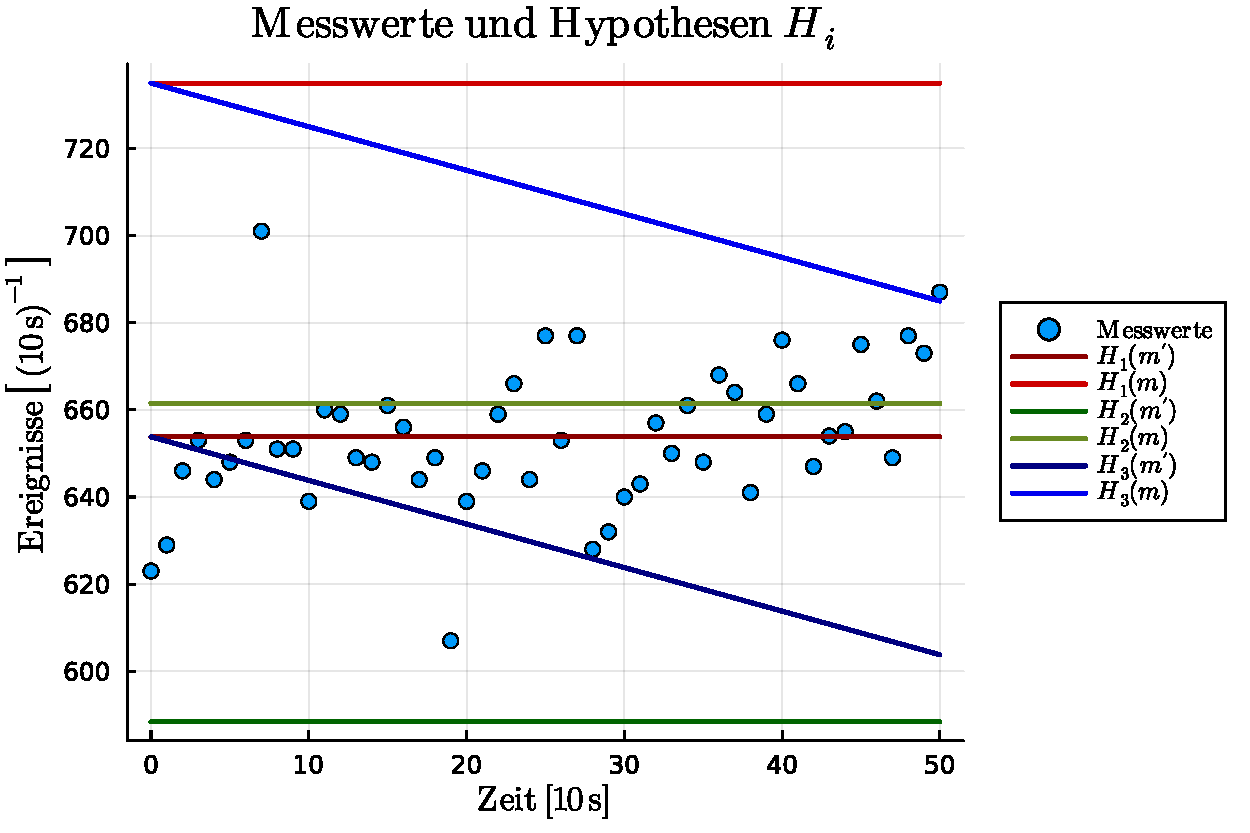
\includegraphics[width=0.7\textwidth]{../media/B3.1/Hypothesen_plot.pdf}
	\caption{Visualisierung der Hypothesen sowie der gewählten Messwerte,\\
		jeweils für gemessene Mittelwerte $m$ und totzeitkorrigierte Mittelwerte $m^\prime$}
	\label{abb:Hypothesen}
\end{figure}

\newpage
\subsubsection{$\chi^2$--Werte}
Nun müssen die einzelnen $\chi^2_i$--Werte für die Hypothesen $H_i$ ermittelt werden. Dazu werden die Summen nach Gleichung \eqref{ChiSquared} gebildet. Für die Hypothesen $H_2$ und $H_3$ muss der Mittelwert entsprechend angepasst werden, wodurch folgende Relationen entstehen.

\begin{eqnarray}
	\bar x &\in& \{m, m^\prime\} \\
	\chi^2_1 &=& \sum_i \frac{(x_i-\bar x_1)^2}{\bar x_1} \\
	\chi^2_2 &=& \sum_i \frac{(x_i-0.9\,\bar x)^2}{0.9\,\bar x} \\
	\chi^2_3 &=& \sum_i \frac{(x_i-(\bar{x} - i))^2}{(\bar{x} - i)}
\end{eqnarray}

\noindent
Die daraus folgenden Ergebnisse werden in Tabelle \ref{tab:ChiSquared} dargestellt. Alle Hypothesen müssen abgelehnt werden. Allerdings gibt es zwei Hypothesen, namentlich $H_1(m^\prime)$ und $H_2(m)$, bei denen der Minimalwert $\chi^2_\mathrm{min}$ unterschritten wurde. Im Falle von $H_1(m^\prime)$ ist das $\chi^2$ um ca. $36\,\%$ kleiner. Im Fall von $H_2(m)$ ist das $\chi^2$ dagegen nur um ca. $4.36\,\%$ kleiner.

Damit lässt sich schließen, dass $H_2$ für einen totzeitkorrigierten Mittelwert am ehesten bekräftigen lässt.

\begin{table}[h]
	\centering
	\begin{tabular}{c|c|c|c|c|c}
		$H_1(m^\prime)$
			& $H_1(m)$
			& $H_2(m^\prime)$
			& $H_2(m)$
			& $H_3(m^\prime)$
			& $H_3(m)$
			\\
		\hline
		$20.84$
			& $475.73$
			& $393.64$
			& $25.14$
			& $106.02$
			& $270.52$
			\\
		$\chi^2 < \chi^2_\mathrm{min}$
			& $\chi^2 \gg \chi^2_\mathrm{max}$
			& $\chi^2 \gg \chi^2_\mathrm{max}$
			& $\chi^2 < \chi^2_\mathrm{min}$
			& $\chi^2 > \chi^2_\mathrm{min}$
			& $\chi^2 \gg \chi^2_\mathrm{min}$
			\\
		$\chi^2 < \chi_\mathrm{P, max}^2$
			& $\chi^2 \gg \chi_\mathrm{P, max}^2$
			& $\chi^2 \gg \chi_\mathrm{P, max}^2$
			& $\chi^2 < \chi_\mathrm{P, max}^2$
			& $\chi^2 > \chi_\mathrm{P, max}^2$
			& $\chi^2 \gg \chi_\mathrm{P, max}^2$
	\end{tabular}
	\caption{Ergebnisse des $\chi^2$--Tests mit $\chi^2_\mathrm{min} = 32.357$ und $\chi^2_\mathrm{max} = 71.420$ \cite{Kapur}}
	\label{tab:ChiSquared}
\end{table}

\noindent
Würde man stattdessen Pearsons $\chi^2$--Test\footnote{Siehe Abschnitt \ref{pearsons-chi2test}} durchführen, so würde man nur einen einzelnen Wert $\chi_\mathrm{P, max}^2 = 67.505$ zum Vergleich verwenden. \cite{Kapur} In diesem Falle würden die Hypothesen $H_1(m^\prime)$ und $H_2(m)$ bekräftigt werden, während die anderen Hypothesen verworfen werden.

Damit könnte man aus den Ergebnissen schließen, dass die Präparatstärke im gemessenen Zeitrahmen konstant ist. Diese Konstante entspricht dem gemessenen Mittelwert $m^\prime$, der etwa $10\,\%$ kleiner als der totzeitkorrigierte Mittelwert $m$ ist.

\hypertarget{totzeit}{\subsubsection{Halbwertszeit}\label{totzeit}}
Die Hypothese $H_3$ nähert den exponentiellen Abfall der Präparatstärke linear an. Wie schon in Abschnitt \ref{Hypothesen} erläutert wurde, ist dies für den beobachteten Messzeitraum nicht beobachtbar, was auch der $\chi^2$--Test bekräftigt.

Dennoch ist die Näherung im Allgemeinen sinnvoll. Die Halbwertszeit der $\ce{^{137}Cs}$--Probe von ca. $T_\mathrm{Cs}=30$ Jahren \cite{Chart of Nuclides}  zu groß, um in unseren Messungen einen (linearen) Abfall der Präparatstärke zu beobachten, so die These.

Im Folgenden soll angenommen werden, Hypothese $H_3$ treffe zu. Dann kann die Halbwertszeit der Probe $T_{1/2}$ aus der Steigung des beobachteten Abfalls ermittelt werden.

Hierzu wird die Präperatsstärke durch die Anzahl der nicht--zerfallenen Atome $N(t)$ beschrieben. Nach Hypothese $H_3$ sei die Präperatsstärke zum Zeitpunkt $t=0$ identisch mit dem gemessenen Mittelwert. Daraus folgt Gleichung \eqref{eq:HWZ 1}.

Weiterhin soll $N(\Delta t)$ nach $\Delta t=10\mathrm{\,s}$ um $1$ geringer als $N(0)$ sein, was durch Gleichung \eqref{eq:HWZ 2} beschrieben wird. Damit kann die Zerfallswahrscheinlichkeit $\lambda$ bestimmt werden. Folglich erhält man die Halbwertszeit nach Gleichung \eqref{eq:Zerfallswahrscheinlichkeit}.

\begin{align}
	N(t) =& m \cdot \exp[-\lambda t] \label{eq:HWZ 1}\\
	N(\Delta t) =& m-1 \\
	m-1 =& m \cdot \exp[-\lambda \Delta t] \label{eq:HWZ 2}\\
	\lambda =& \frac{1}{\Delta t} \ln(\frac{m}{m-1}) \\
	T_{1/2}(m) =& \frac{\Delta t \ln(2)}{\ln(\frac{m}{m-1})}
\end{align}

\noindent
Auf diese Weise erhält man eine Halbwertszeit von $T_{1/2}(m^\prime)=1\,\mathrm{h}\,28\,\mathrm{min}\lll T_\mathrm{Cs}$ und eine totzeitkorrigierte Halbwertszeit von $T_{1/2}(m)=1\,\mathrm{h}\,51\,\mathrm{min}\lll T_\mathrm{Cs}$. Beide Halbwertszeiten verschwinden im Vergleich zu der Halbwertszeit von $\ce{^{137}Cs}$.

Zudem gibt es ein weiteres systematisches Problem. Nach $H_3$ soll $N(0)$ dem Mittelwert aller Messwerte entsprechen. Bei linear abfallenden Werten dürfte dieser Mittelwert in etwa dem Wert nach der halben Messdauer entsprechen. Stattdessen müsste man den Mittelwert der ersten Werte verwenden.

Daher könnte man die Halbwertszeit auf diese Weise messen, allerdings nur bei Proben, die eine deutlich kürzere Halbwertszeit als $\ce{^{137}Cs}$ haben. Dabei muss man allerdings einen anderen Startwert $N(0)$ als in der Hypothese $H_3$ wählen.

\clearpage
\hypertarget{fazit}{%
\section{Fazit}\label{fazit}}
Zusammenfassend scheint das Experiment erfolgreich gewesen zu sein. Die Darstellungen der Messwerte durch die Verteilungen ist gut gelungen, die $\chi^2$--Tests haben akzeptable Ergebnisse geliefert. Nur die Bestimmung der Totzeit scheint teilweise recht ungenau zu sein.

So lange man nicht zu viele Ereignisse misst, kann man die Verteilung sowohl mit einer Poisson--Verteilung als auch einer Gauß--Verteilung darstellen. Bis zu einer gewissen Menge von Ereignissen ist die Poisson--Verteilung sinnvoller zu verwenden, danach die Gauß--Verteilung.

Dies bestätigt den Satz von Moivre--Laplace, nach dem eine Binomialverteilung ab einer Standardabweichung von $9$ durch eine Gauß--Verteilung beschrieben werden kann. Auch dass die Poisson--Verteilung als Grenzfall der Binomialverteilung folgen kann, wurde auf diese Weise bestätigt.

Die Totzeit mithilfe der Zwei--Präperate--Methode zu bestimmen ist rechnerisch aufwendig, allerdings gut machbar. Allerdings sind die manuell errechneten Fehler sehr hoch, bei mindestens $50\,\%$ und bis zu ca. $370\,\%$. Auch wenn man die Fehler direkt von einer Software berechnen kann, sind die relativen Fehler $\tau_1=1\mathrm{\,ms}-6\mathrm{\,ms}$ sehr hoch. Bei $\tau_2>18\mathrm{\,ms}$ dagegen sind die Ungenauigkeiten deutlich geringer.

Ein weiteres Problem liefert der Umstand, dass es zwei rechnerisch mögliche Totzeiten gibt. Allerdings kann es physikalisch nur eine Totzeit geben, da diese eine Eigenschaft des Detektors beschreibt. Daher sollte die Totzeit auch auf eine andere Methode bestimmt werden, um die richtige Totzeit finden. Dafür bietet sich die Analyse einer Invervallverteilung der Messwerte an.

Die $\chi^2$--Tests begründen eine Ablehnung aller drei getätigten Hypothesen. Allerdings sind sie dennoch aussagekräftig: Nur die Möglichkeit, dass Präperatsstärke von $\ce{^{137}Cs}$ im Zeitraum von Minuten konstant bleibt, kann durch die Tests unterstützt werden. Bei dem $\chi^2$--Test nach Pearson wird diese These eindeutig bekräftigt.

Hierbei kann der gemessene Mittelwert der Messwerte als konstanter Wert angenommen werden. Dieser ist allerdings durch die Totzeit um ca. $10\,\%$ kleiner als der tatsächliche Mittelwert.

Zuletzt wurde die Halbwertszeit einer Probe ermittelt, die zu Beginn die selbe Präperatsstärke wie unsere Probe hat, bei der dagegen ein linearer Abfall zu beobachten wäre. Um den in der dritten Hypothese beschriebene Steigung zu erhalten, ist eine Halbwertszeit von ca. $1.5\mathrm{\,h}-2\mathrm{\,h}$ benötigt.

\clearpage
\hypertarget{literatur}{\section{Literaturverzeichnis}\label{literatur}}
\renewcommand{\section}[2]{}

\begin{thebibliography}{99}
\bibitem{Statistical Inference}
	G. Casella, R. L. Berger, ``Statistical Inference'', ISBN~9781003456285,
	DOI~\href{https://doi.org/10.1201/9781003456285}{10.1201/9781003456285}
\bibitem{Gigerenzer}
	G. Gigerenzer, ``Mindless statistics'', 2004, \emph{The Journal of
		Socio--Economics},
		DOI~\href{https://doi.org/10.1016/j.socec.2004.09.033}{0.1016/j.socec.2004.09.033}
\bibitem{Cramer} % unlinked
	E. Cramer \& U. Kamps, ``Grundlagen der Wahrscheinlichkeitsrechnung
	und Statistik'', Springer 2020, DOI~\href{https://doi.org/10.1007/978-3-662-60552-3}{10.1007/978-3-662-60552-3}
\bibitem{Puhani} % unlinked
	J. Puhani, ``Statistik'', Springer 2020, DOI~\href{https://doi.org/10.1007/978-3-658-28955-3}{10.1007/978-3-658-28955-3}
\bibitem{McHugh}
	Mary L. McHugh, ``The Chi-square test of independence'', Biochemia Medica, DOI~\href{https://doi.org/10.11613/BM.2013.018}{10.11613/BM.2013.018}
\bibitem{Kapur}
	K. C. Kapur \& M. Pecht, ``Reliability Engineering'': Appendix E,
	Wiley 2014,
	DOI~\href{https://doi.org/10.1002/9781118841716}{10.1002/9781118841716}
\bibitem{uni}
	Universität zu Köln, ``B3.1: Statistik der Kernzerfälle'', Januar
	2021, Online verfügbar unter
	\url{https://www.ikp.uni-koeln.de/fileadmin/data/praktikum/B3.1_statistik_de.pdf}, Abruf am 10.04.2024
\bibitem{Halbwertszeit}
	Lexikon der Physik, ``Halbwertszeit'', \url{https://www.spektrum.de/lexikon/physik/halbwertszeit/6327}, Abruf am 07.06.2024
\bibitem{Chart of Nuclides}
	National Nuclear Data Center, ``Chart of Nuclides'',
	\url{https://www.nndc.bnl.gov/nudat3}, $\ce{^{137}Cs}$,
	Abruf am 07.05.2024
\bibitem{ulfkonrad}
	Ulf Konrad, ``Geiger--Müller--Zählrohr'', \url{https://www.ulfkonrad.de/physik/geiger-mueller-zaehlrohr}, Abruf am 22.04.2024
\bibitem{Totzeit}
	Lexikon der Physik, ``Totzeit'', \url{https://www.spektrum.de/lexikon/physik/totzeit/14643}, Abruf am 22.04.2024
\bibitem{File:Geigerzählrohr}
	Wikimedia, ``File:Geiger Mueller Counter with Circuit-de.svg'', \url{https://commons.wikimedia.org/wiki/File:Geiger_Mueller_Counter_with_Circuit-de.svg}, Abruf am 22.04.2024
\bibitem{Julia:Measurements}
	\code{\href{https://julialang.org}{Julia}}--Paket \code{Measurements}, Dokumentation unter \url{https://juliaphysics.github.io/Measurements.jl/stable}
\end{thebibliography}
\end{document}
